\documentclass[11pt,a4paper]{article}
\usepackage{fontspec}
\setmainfont{texgyretermes}[Extension=.otf,UprightFont=*-regular,BoldFont=*-bold,ItalicFont=*-italic,BoldItalicFont=*-bolditalic]
\setsansfont{texgyreheros}[Extension=.otf,UprightFont=*-regular,BoldFont=*-bold,ItalicFont=*-italic,BoldItalicFont=*-bolditalic]
\setmonofont{lmmono10}[Extension=.otf,UprightFont=*-regular]
\usepackage[a4paper,margin=2.2cm]{geometry}
\usepackage{graphicx,booktabs,tabularx,array,amsmath,amssymb,float,enumitem,xcolor}
\usepackage[font=small,labelfont=bf]{caption}
\usepackage[most]{tcolorbox}
\usepackage[colorlinks=true,linkcolor=teal!60!black,urlcolor=teal!60!black,citecolor=teal!60!black]{hyperref}
\usepackage{titlesec}
\usepackage{tikz}
\usetikzlibrary{positioning,arrows.meta,calc}

\definecolor{acc}{HTML}{2A78D6}
\definecolor{org}{HTML}{EB6834}
\titleformat{\section}{\Large\sffamily\bfseries\color{acc!75!black}}{\thesection}{0.6em}{}
\titleformat{\subsection}{\large\sffamily\bfseries}{\thesubsection}{0.5em}{}
\titlespacing*{\section}{0pt}{12pt}{5pt}
\titlespacing*{\subsection}{0pt}{8pt}{3pt}
\setlist{itemsep=2pt,topsep=3pt}
\renewcommand{\arraystretch}{1.18}
\newtcolorbox{ghichu}[1][Điểm cần nhớ]{colback=acc!5,colframe=acc!70!black,fonttitle=\sffamily\bfseries,title=#1,
  boxrule=0.6pt,arc=2pt,left=6pt,right=6pt,top=4pt,bottom=4pt}
\captionsetup{justification=raggedright,singlelinecheck=false}
\graphicspath{{figs/}}
\renewcommand{\figurename}{Hình}
\renewcommand{\tablename}{Bảng}
\renewcommand{\refname}{Tài liệu tham khảo}
\renewcommand{\abstractname}{Tóm tắt}
\setcounter{topnumber}{3}\setcounter{totalnumber}{4}\renewcommand{\topfraction}{0.9}\renewcommand{\textfraction}{0.1}\renewcommand{\floatpagefraction}{0.8}
\newcommand{\OKS}{\mathrm{OKS}}

\begin{document}

\begin{center}
{\sffamily\bfseries\LARGE Mỗi người một dự đoán: điểm tin cậy đáng giá bao nhiêu\\[2pt] với OKS AP trên camera giám sát chưa thấy}\\[8pt]
{\large Báo cáo kỹ thuật, UPAR Challenge 2027, Track 3 (2D Human Pose Estimation)}\\[6pt]
{\small Tài khoản Codabench \texttt{tannguyenbmt47} \quad Cập nhật ngày 06/10/2026}
\end{center}

\begin{abstract}
\noindent Khi khung người được cho sẵn, một mô hình ước lượng tư thế top-down đưa ra đúng một dự đoán cho mỗi người, và OKS AP của COCO khi đó phụ thuộc vào hai thứ: mỗi dự đoán chính xác đến đâu, và \textbf{điểm tin cậy} (confidence score) xếp các dự đoán theo đúng thứ tự đến đâu. Chúng tôi chỉ ra rằng trong tình huống này, AP ở mỗi ngưỡng OKS nằm giữa $f_t^2$ và $f_t$, với $f_t$ là tỉ lệ dự đoán đúng, và hai cận này khớp với AP của một điểm không chứa thông tin và của một điểm hoàn hảo trên dữ liệu thật. Chúng tôi đo cả hai yếu tố trên UPAR 2027 Track~3 với các mô hình ViTPose++ được đánh giá trên bộ dữ liệu giấu. Giữ nguyên toạ độ khớp, một điểm tin cậy hoàn hảo sẽ thêm 1,3 đến 1,5 điểm AP, nhiều hơn việc gộp heatmap của mô hình thứ hai (0,1 đến 0,5 điểm). Phần lớn giá trị này nằm ở việc tách dự đoán rất tốt khỏi dự đoán tốt, ở ngưỡng OKS 0.95, chứ không ở việc đẩy các dự đoán hỏng xuống cuối. Điểm mặc định, trung bình các cực đại heatmap, tính cả hai kênh tai, vốn không bao giờ được gán nhãn trong định dạng này. Bỏ hai kênh đó đã lấy lại phần lớn mức tăng của một bộ chấm cây tăng cường học trên thống kê heatmap, còn chính bộ chấm đó, được kiểm chứng giấu bộ dữ liệu ở cả hai tầng, lấy lại 12 đến 30\% mức tăng của điểm lý tưởng. Trên tập chấm, nó thêm 0,15 điểm, nằm trong khoảng dự báo từ miền giấu. Hai phép đo nữa thay đổi cách nhìn về nguồn lỗi. Tinh chỉnh trông như đáng giá 23 điểm, nhưng trên các khớp chung của COCO và PoseTrack nó chỉ đáng 0,7 điểm, nên phần lớn mức tăng đó là học định nghĩa điểm khớp vùng đầu. Và lỗi nhầm trái phải chỉ ảnh hưởng 1,3\% số người trong PETA, nhưng sửa được chúng sẽ thêm 1,65 điểm, nhiều hơn cả một điểm tin cậy hoàn hảo. Hệ thống đạt 0.8992 AP trên tập chấm ẩn, so với 0.8813 của một mô hình ViTPose++ base tinh chỉnh.
\end{abstract}

\tableofcontents
\newpage

%=====================================================================
\section{Giới thiệu}

Ước lượng tư thế người 2D xác định toạ độ các điểm khớp như vai, khuỷu tay, hông, đầu gối trên ảnh. Trong giám sát, tư thế là đầu vào cho nhận dạng hành động, theo vết người qua nhiều camera và phân tích hành vi. Các hệ thống hiện đại theo cách tiếp cận top-down đạt độ chính xác cao trên các bộ dữ liệu chuẩn như COCO~\cite{coco}. Một bộ dò người tìm khung bao, rồi một mạng ước lượng tư thế xử lý từng khung~\cite{simplebaseline,hrnet,vitpose}.

Ảnh giám sát khác COCO ở ba điểm. Người trong ảnh nhỏ: trung vị chiều cao khung là 149 pixel ở PETA, 205 ở PA100k và 128 ở Market1501. Ảnh mờ, nén mạnh và có màu lệch. Góc nhìn từ trên cao và người hay bị che khuất bởi người khác. Track 3 của UPAR Challenge 2027 đánh giá đúng tình huống này. Khung người được cho sẵn, nên bài toán chỉ còn bước ước lượng tư thế, nhưng tập chấm lấy từ một miền camera không có trong dữ liệu huấn luyện.

Vì khung người được cho sẵn, mỗi người nhận đúng một dự đoán. Điều đó thay đổi thứ mà chỉ số thưởng: điểm tin cậy không còn chọn giữa nhiều tư thế ứng viên, mà chỉ quyết định thứ tự duyệt một tập dự đoán cố định. Báo cáo đo phần giá trị này, thiết kế một điểm tin cậy dựa trên phép đo đó, và hỏi lỗi còn lại nằm ở đâu. Các đóng góp chính gồm bốn điểm.

\begin{enumerate}[leftmargin=1.4em]
\item Một phân tích AP khi mỗi khung có một dự đoán, với hai cận $f_t^2$ và $f_t$ được kiểm chứng trên dữ liệu giấu (mục~\ref{sec:metric}).
\item Một phép đo giá trị của điểm tin cậy theo từng bộ dữ liệu và từng ngưỡng, cho thấy giá trị chủ yếu nằm ở việc sắp các dự đoán tốt, không ở việc loại các dự đoán hỏng (mục~\ref{sec:score}).
\item Một bộ chấm lại điểm tin cậy được kiểm chứng giấu bộ dữ liệu ở cả hai tầng, cùng phát hiện rằng chỉ cần bỏ hai kênh tai khỏi điểm mặc định đã thu được phần lớn lợi ích của nó (mục~\ref{sec:rescore}).
\item Hai điều chỉnh cho cách đọc quen thuộc: phần lớn mức tăng của tinh chỉnh là hiệu ứng định nghĩa điểm khớp, và lỗi nhầm trái phải tốn nhiều AP hơn cả khoảng cách tới điểm tin cậy lý tưởng trên PETA (mục~\ref{sec:lodo} và~\ref{sec:errors}).
\end{enumerate}

%=====================================================================
\section{Bài toán và chỉ số đánh giá}
\label{sec:task}

\subsection{Dữ liệu}

Mỗi mẫu gồm một ảnh và một hoặc nhiều khung người. Với mỗi khung, chương trình phải trả về toạ độ của 17 điểm khớp theo định dạng PoseTrack18~\cite{posetrack}, gồm mũi, đáy đầu, đỉnh đầu, hai tai, hai vai, hai khuỷu tay, hai cổ tay, hai hông, hai đầu gối và hai cổ chân, cùng một điểm tin cậy cho cả người. Hai điểm tai được giữ trong định dạng nhưng không có nhãn và không được chấm.

Ban tổ chức cung cấp nhãn tư thế cho ảnh của ba bộ dữ liệu UPAR (Bảng~\ref{tab:data}). Ảnh có độ phân giải thấp, đặc biệt ở PETA và Market1501, và mỗi ảnh là một khung cắt quanh một người, đôi khi có người khác xuất hiện một phần.

\begin{table}[H]
\centering\small
\begin{tabular}{@{}lrrl@{}}
\toprule
Bộ dữ liệu & Số ảnh & Số người có nhãn & Ghi chú \\
\midrule
PA100k & 19.500 & 19.499 & ngoài trời, nhiều camera \\
Market1501 & 12.924 & 12.923 & một khu mua sắm, ảnh 128×64 \\
PETA & 10.402 & 10.314 & gộp 10 nguồn ảnh, độ phân giải và chất lượng không đều \\
\midrule
Tổng & 42.826 & 42.736 & \\
\bottomrule
\end{tabular}
\caption{Dữ liệu tư thế của Track 3. Chỉ những người có ít nhất một điểm khớp được gán nhãn được dùng để huấn luyện và đánh giá.}
\label{tab:data}
\end{table}

\subsection{OKS AP}
\label{sec:metric}

\paragraph{OKS.} Độ tương đồng điểm khớp (object keypoint similarity) so dự đoán $\hat x$ với nhãn $x$ của một người:
\begin{equation}
\OKS=\frac{\sum_{k}\exp\!\left(-\dfrac{\|\hat x_k-x_k\|^2}{2\,s^2\,\kappa_k^2}\right)\mathbb{1}[v_k>0]}{\sum_k\mathbb{1}[v_k>0]},
\end{equation}
với $s^2$ là diện tích của người, $\kappa_k=2\sigma_k$ là hằng số của khớp $k$, và $v_k$ cho biết khớp $k$ có nhãn hay không. Hằng số $\sigma_k$ lấy theo COCO, riêng đáy đầu và đỉnh đầu dùng giá trị của mắt theo quy ước PoseTrack. OKS bằng 1 khi mọi khớp trùng nhãn và giảm theo bình phương khoảng cách chuẩn hoá theo kích thước người. Khớp có $\sigma$ nhỏ như mũi bị phạt nặng hơn khớp có $\sigma$ lớn như hông.

\paragraph{AP.} Với một ngưỡng $t$, một dự đoán được coi là đúng nếu OKS của nó với nhãn vượt $t$. Mọi dự đoán của toàn tập chấm được xếp theo điểm tin cậy giảm dần, rồi precision và recall được tính dọc theo danh sách đó. AP ở ngưỡng $t$ là diện tích dưới đường precision theo recall. OKS AP là trung bình của AP ở 10 ngưỡng $t\in\{0.50,0.55,\dots,0.95\}$~\cite{coco}.

\paragraph{Vai trò của điểm tin cậy.} Trong bài toán này mỗi khung có đúng một người và một dự đoán. Nếu điểm tin cậy được sắp đúng theo OKS, mọi dự đoán đúng ở ngưỡng $t$ đứng trước mọi dự đoán sai. Precision khi đó bằng 1 cho tới khi hết dự đoán đúng, và AP ở ngưỡng $t$ bằng tỉ lệ dự đoán đúng $f_t$. Nếu điểm tin cậy không chứa thông tin, dự đoán đúng và sai xen kẽ ngẫu nhiên, precision ở mọi độ sâu xấp xỉ $f_t$, và AP xấp xỉ $f_t^2$. Với $f_t=0.8$, khoảng cách giữa hai trường hợp là 0.16. Vì vậy cùng một tập toạ độ khớp có thể cho AP khác nhau đáng kể tuỳ cách gán điểm tin cậy.

Bảng~\ref{tab:bounds} kiểm tra hai cận trên dự đoán của mô hình huge giấu từng bộ dữ liệu. Trung bình của $f_t^2$ cách AP của điểm hằng số không quá nửa điểm ở cả ba bộ. Trung bình của $f_t$ cao hơn AP của điểm lý tưởng khoảng 0.4 đến 0.5 điểm, do cách nội suy 101 điểm của COCO. Hai cận cũng cho thấy điểm tin cậy có thể quan trọng ở đâu: $f_t$ còn ít nhất 0.95 ở mọi ngưỡng tới 0.85, rồi giảm còn 0.69 đến 0.76 ở 0.95.

\begin{table}[H]
\centering\small
\begin{tabular}{@{}lccc@{}}
\toprule
Bộ giấu & PETA & PA100k & Market1501 \\
\midrule
$f_{0.50}$ / $f_{0.85}$ / $f_{0.95}$ & 0.991 / 0.950 / 0.759 & 0.990 / 0.961 / 0.690 & 0.998 / 0.972 / 0.705 \\
trung bình $f_t^2$ & 0.9041 & 0.9033 & 0.9241 \\
AP, điểm hằng số & 0.9050 & 0.9006 & 0.9200 \\
trung bình $f_t$ & 0.9485 & 0.9464 & 0.9574 \\
AP, OKS thật làm điểm & 0.9436 & 0.9426 & 0.9525 \\
\bottomrule
\end{tabular}
\caption{Hai cận của chế độ một dự đoán cho mỗi người, so với AP đo được (mô hình huge, giữ nguyên toạ độ khớp).}
\label{tab:bounds}
\end{table}

\subsection{Ràng buộc và luật thi}

Bài nộp là chương trình. Máy chấm có GPU và cho phép tối đa 7200 giây cho 30.245 khung người. Môi trường chấm có PyTorch 2.4.1, numpy và Pillow, không có OpenCV, scikit-learn hay mạng. Luật thi cho phép tiền huấn luyện trên COCO và PoseTrack18, cấm dữ liệu tiền huấn luyện ngoài và mô hình nền tảng, và cấm dùng ảnh chấm cho huấn luyện, gán nhãn giả hay chọn siêu tham số. Ban tổ chức cung cấp một bài mẫu dùng ViTPose+ small không tinh chỉnh, đạt 0.6238 trên tập chấm. Các checkpoint ViTPose+ công khai được huấn luyện trên nhiều bộ dữ liệu tư thế và khởi tạo từ MAE trên ImageNet. Chúng tôi dùng họ mô hình này vì bài mẫu chính thức của ban tổ chức dùng nó, và hiểu đó là sự cho phép; nếu cách hiểu này sai, kết quả của chúng tôi sẽ không hợp lệ. Vì cùng lý do luật thi, chúng tôi không dùng DINOv3 hay chưng cất từ bất kỳ mô hình nền tảng nào cho track này.

\begin{ghichu}
OKS AP đo hai thứ cùng lúc, gồm độ chính xác của toạ độ khớp và khả năng của điểm tin cậy trong việc xếp dự đoán tốt lên trước dự đoán kém. Thành phần thứ hai thường bị bỏ qua, nhưng nó cải thiện được mà không cần đụng vào mô hình tư thế.
\end{ghichu}

%=====================================================================
\section{Nghiên cứu liên quan}

\paragraph{Ước lượng tư thế top-down dựa trên heatmap.} SimpleBaseline~\cite{simplebaseline} dùng backbone ResNet và các lớp giải chập để dự đoán một heatmap cho mỗi khớp. HRNet~\cite{hrnet} giữ biểu diễn độ phân giải cao suốt mạng. ViTPose~\cite{vitpose} dùng một Vision Transformer thuần với decoder nhẹ, khởi tạo từ MAE~\cite{mae}, và đạt độ chính xác cao nhất trên COCO trong họ heatmap. ViTPose+~\cite{vitposepp} huấn luyện chung trên nhiều bộ dữ liệu tư thế với các head riêng theo bộ dữ liệu trên một backbone dùng chung.

\paragraph{Mã hoá và giải mã heatmap.} UDP~\cite{udp} chỉ ra sai lệch hệ thống trong các phép biến đổi toạ độ giữa ảnh, khung cắt và heatmap, và đề xuất dùng quy ước tâm pixel. DARK~\cite{dark} giải mã toạ độ dưới mức ô lưới bằng khai triển Taylor bậc hai của logarit heatmap đã làm mượt, thay cho phép dời một phần tư ô truyền thống. Chúng tôi dùng cả hai.

\paragraph{Điểm tin cậy của dự đoán tư thế.} Papandreou và cộng sự~\cite{gpose} tính điểm tin cậy của một người từ các cực đại heatmap thay vì chỉ dùng điểm của bộ dò người. Ronchi và Perona~\cite{ronchi} phân tích lỗi của OKS AP và chỉ ra rằng điểm tin cậy kém hiệu chỉnh là một nguồn mất AP đáng kể. Gần đây, Gu và cộng sự~\cite{ccnet} đề xuất CCNet, một nhánh nhẹ dự đoán OKS từ đặc trưng của mạng tư thế, tăng 0.8 AP cho ViTPose-B trên COCO mà không huấn luyện lại mô hình chính. DEKR~\cite{dekr} cũng huấn luyện một mạng nhỏ trên toạ độ dự đoán để ước lượng OKS. Phương pháp của chúng tôi cùng ý tưởng nhưng chỉ dùng thống kê của heatmap đầu ra, nên chạy được bên ngoài mô hình đã đóng gói, và được kiểm chứng trên miền giấu thay vì trên phân bố huấn luyện.

\paragraph{Tổng quát hoá miền cho tư thế.} Các công trình thích nghi miền cho tư thế thường dùng ảnh không nhãn của miền đích để gán nhãn giả và tự huấn luyện. Luật thi cấm dùng ảnh chấm theo cách này, nên chúng tôi không đi theo hướng đó.

%=====================================================================
\section{Phương pháp}
\label{sec:method}

\subsection{Tổng quan}

Hình~\ref{fig:pipe} tóm tắt hệ thống của bài nộp tốt nhất (v6). Mỗi khung người được cắt và đưa về 256×192. Hai mô hình ViTPose+ (large và huge) chạy trên ảnh và ảnh lật ngang. Heatmap được lấy trung bình rồi giải mã bằng DARK thành 17 toạ độ. Song song, một bộ đặc trưng tính từ chính các heatmap đó được đưa vào một bộ hồi quy cây để ước lượng OKS, và ước lượng này trở thành điểm tin cậy.

\begin{figure}[H]
\centering
\begin{tikzpicture}[font=\sffamily\scriptsize, node distance=4mm and 4.5mm,
  box/.style={draw=black!55, rounded corners=2pt, fill=white, align=center, minimum height=8mm, inner sep=3pt},
  hl/.style={box, fill=acc!10, draw=acc!80!black},
  tc/.style={box, fill=org!10, draw=org!80!black},
  arr/.style={-{Latex[length=2mm]}, black!65}]
\node[box] (img) {Ảnh + khung\\ người};
\node[box, right=of img] (crop) {Cắt affine\\ đệm 1.25\\ 256×192};
\node[hl, right=of crop, yshift=5mm] (l) {ViTPose+ L\\ ảnh + ảnh lật};
\node[hl, right=of crop, yshift=-7mm] (h) {ViTPose+ H\\ ảnh + ảnh lật};
\node[box, right=of l, yshift=-6mm] (avg) {Trung bình\\ heatmap\\ 17×64×48};
\node[box, right=of avg, yshift=6mm] (dark) {Giải mã DARK\\ $\to$ 17 toạ độ};
\node[tc, right=of avg, yshift=-8mm] (feat) {87 đặc trưng\\ heatmap};
\node[tc, right=of feat] (gbm) {150 cây\\ $\to\widehat{\OKS}$};
\node[box, right=of dark] (kp) {Toạ độ khớp};
\node[box, right=of gbm] (sc) {Điểm tin cậy};
\draw[arr] (img)--(crop); \draw[arr] (crop.east)--(l.west); \draw[arr] (crop.east)--(h.west);
\draw[arr] (l.east)--(avg.west); \draw[arr] (h.east)--(avg.west);
\draw[arr] (avg.east)--(dark.west); \draw[arr] (avg.east)--(feat.west); \draw[arr] (feat)--(gbm);
\draw[arr] (dark)--(kp); \draw[arr] (gbm)--(sc);
\draw[arr, dashed] (l.north east) to[out=20,in=150] (feat.north);
\draw[arr, dashed] (h.east) to[out=-10,in=200] (feat.south west);
\end{tikzpicture}
\caption{Hệ thống Track 3 (bài nộp v6). Nhánh xanh tạo toạ độ khớp và giống hệt bài nộp v3. Nhánh cam chỉ thay điểm tin cậy. Đường đứt nét là các đặc trưng dùng heatmap riêng của từng mô hình, như độ lệch giữa toạ độ của large và huge.}
\label{fig:pipe}
\end{figure}

\subsection{Mô hình tư thế}
\label{sec:model}

\paragraph{Lựa chọn.} Chúng tôi dùng ViTPose+~\cite{vitposepp}, cùng họ mô hình với bài mẫu của ban tổ chức, ở bốn cỡ small, base, large và huge. Backbone là ViT với patch 16×16, ảnh vào 256×192 cho 16×12 token, và một decoder nhẹ biến token thành 17 heatmap kích thước 64×48. ViTPose+ có các thành phần riêng theo từng bộ dữ liệu tiền huấn luyện, được chọn bằng một chỉ số bộ dữ liệu. Chúng tôi dùng chỉ số của COCO. COCO và PoseTrack18 dùng chung 15 điểm (mũi, hai tai và 12 khớp cơ thể) và chỉ khác nhau ở vùng đầu, nên head COCO là điểm khởi đầu gần nhất.

\paragraph{Ánh xạ khung sang ảnh vào.} Khung người $(x,y,w,h)$ được mở rộng về tỉ lệ 3:4 bằng cách kéo dài cạnh ngắn, rồi nhân kích thước với hệ số đệm 1.25 để giữ ngữ cảnh quanh người. Phép affine ánh xạ vùng này sang ảnh 256×192 theo quy ước tâm pixel của UDP~\cite{udp}. Tâm vùng ánh xạ vào $((W-1)/2,(H-1)/2)$ và tỉ lệ là $(W-1)/s_w$. Quy ước này loại bỏ sai lệch nửa pixel giữa ảnh, ảnh vào và heatmap, vốn đáng kể khi người chỉ cao 64 pixel.

\paragraph{Mục tiêu và hàm mất mát.} Mỗi khớp có nhãn tạo một heatmap mục tiêu Gauss với $\sigma=2$ ô lưới tại toạ độ đã ánh xạ. Hàm mất mát là sai số bình phương trung bình giữa heatmap dự đoán và heatmap mục tiêu, nhân với trọng số khả kiến của từng khớp (bằng 0 cho khớp không có nhãn hoặc nằm ngoài khung cắt), rồi nhân 1000 để có độ lớn gradient phù hợp.

\paragraph{Tăng cường dữ liệu.} Khi huấn luyện, kích thước vùng cắt được nhân một hệ số ngẫu nhiên trong $[0.75,1.25]$, tâm được dời tối đa 8\% kích thước, ảnh được xoay với góc lấy từ phân phối Gauss độ lệch chuẩn $30°$, cắt ở $\pm40°$, với xác suất 0.4, lật ngang với xác suất 0.5 (kèm hoán đổi các cặp khớp trái và phải), và với xác suất 0.8 thay đổi độ sáng và độ tương phản.

\paragraph{Huấn luyện.} AdamW, learning rate $5\cdot10^{-5}$ ở tầng cuối với layer decay 0.75, weight decay 0.1 trừ tham số chuẩn hoá và vị trí, warmup 300 bước rồi lịch cosine, batch 64, tính toán bf16. Mô hình nộp bài học 5 epoch trên cả ba bộ dữ liệu. Mô hình thẩm định học 2 epoch trên hai bộ, vì AP trên miền giấu bão hoà sau epoch đầu (Bảng~\ref{tab:epochs}).

\subsection{Suy luận}
\label{sec:infer}

\paragraph{Kiểm tra lật.} Mỗi khung được chạy hai lần, trên ảnh gốc và ảnh lật ngang. Heatmap của ảnh lật được lật lại và hoán đổi các cặp khớp trái và phải, rồi lấy trung bình với heatmap của ảnh gốc.

\paragraph{Gộp mô hình.} Với nhiều mô hình, heatmap đã kiểm tra lật của các mô hình được lấy trung bình trước khi giải mã. Khi hai mô hình bất đồng về vị trí một khớp, heatmap trung bình có hai đỉnh thấp hơn; chúng tôi không so sánh với cách lấy trung bình toạ độ.

\paragraph{Giải mã DARK.} Với mỗi khớp, toạ độ nguyên $m$ là vị trí cực đại của heatmap. Heatmap được làm mượt bằng bộ lọc Gauss kích thước 11 rồi lấy logarit. Toạ độ dưới mức ô lưới là
\begin{equation}
\hat x = m - \big(\nabla^2 \log h(m)\big)^{-1}\,\nabla\log h(m),
\end{equation}
với gradient và Hessian tính bằng sai phân hữu hạn~\cite{dark}. Toạ độ trên heatmap được nhân với tỉ lệ giữa ảnh vào và heatmap, rồi ánh xạ ngược về ảnh gốc bằng nghịch đảo của phép affine. Toàn bộ bước giải mã được viết lại bằng các phép toán tensor của PyTorch để chạy trên GPU, vì môi trường chấm không có OpenCV.

\paragraph{Đóng gói.} Mỗi mô hình được xuất thành TorchScript với trọng số fp16 và chạy trên GPU của máy chấm. Chúng tôi đối chiếu đầu ra của TorchScript với mô hình gốc trên batch ngẫu nhiên trước mỗi lần đóng gói.

%=====================================================================
\section{Giao thức thẩm định và các kết quả về mô hình}
\label{sec:lodo}

\subsection{Giấu từng bộ dữ liệu}

Như ở Track 1 và Track 2, điểm trên dữ liệu đã thấy không dự báo được điểm trên miền mới. Chúng tôi huấn luyện mỗi mô hình thẩm định trên hai bộ dữ liệu và chấm trên toàn bộ người có nhãn của bộ thứ ba, lần lượt với cả ba bộ. Ba mô hình huge và ba mô hình large được huấn luyện theo cách này. Mọi kết quả của mục này và mục~\ref{sec:score} đều tính trên dự đoán của mô hình chưa từng thấy bộ dữ liệu được chấm.

\subsection{Tinh chỉnh là bước quan trọng nhất}

\begin{figure}[H]
\centering
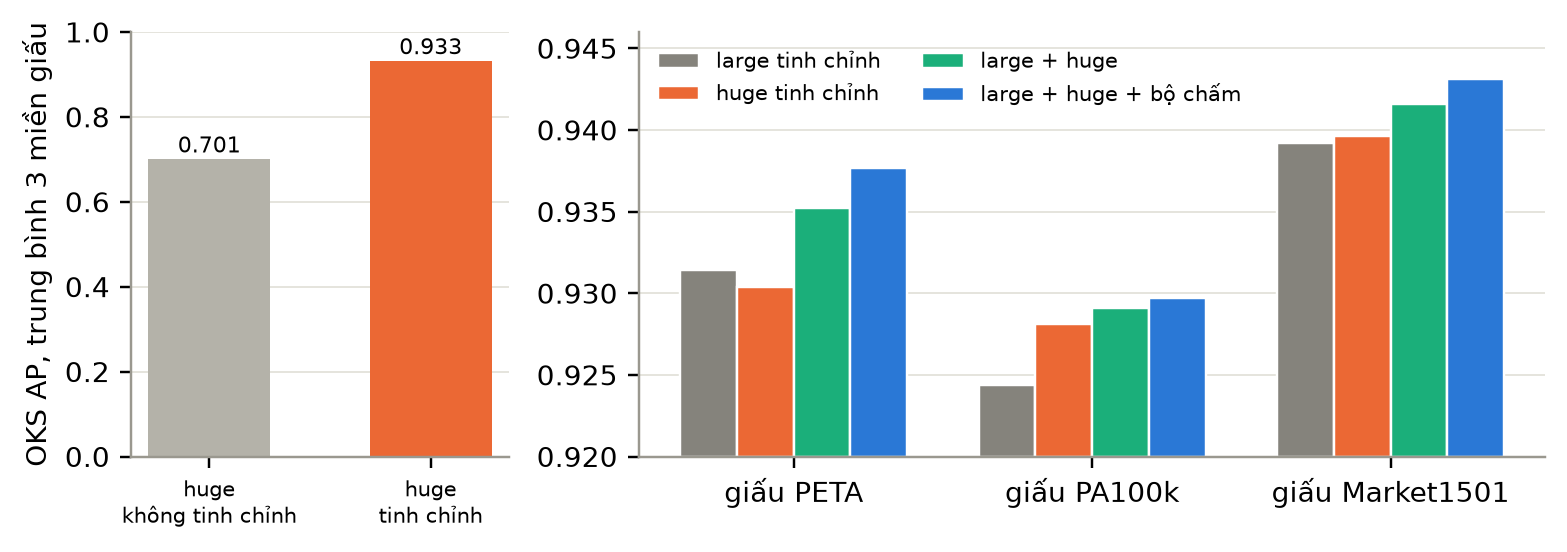
\includegraphics[width=\linewidth]{lodo.png}
\caption{Trái, AP trung bình trên ba miền giấu của ViTPose+ huge trước và sau tinh chỉnh trên dữ liệu UPAR. Phải, AP trên từng miền giấu của large, huge, gộp hai mô hình, và gộp hai mô hình với bộ chấm điểm. Gộp mô hình cho kết quả tốt nhất ở cả ba miền.}
\label{fig:lodo}
\end{figure}

Hình~\ref{fig:lodo} cho thấy ViTPose+ huge không tinh chỉnh chỉ đạt 0.70 AP trên ảnh UPAR, dù đây là mô hình mạnh trên COCO. Sau 2 epoch tinh chỉnh trên hai bộ dữ liệu còn lại, AP trên bộ giấu tăng lên 0.93. Phần lớn khoảng cách này không phải khoảng cách miền ảnh. Mô hình COCO trả về hai mắt ở đúng hai vị trí mà PoseTrack dùng cho đáy đầu và đỉnh đầu, và hai điểm này có hằng số $\sigma$ nhỏ nhất. AP50 của mô hình chưa tinh chỉnh đã là 0.977, tức nó tìm đúng người và chỉ mất điểm ở các ngưỡng chặt, đúng dấu hiệu của một độ lệch có hệ thống. Khi chấm cả hai mô hình chỉ trên 13 khớp chung (bỏ đáy đầu và đỉnh đầu khỏi nhãn), khoảng cách thu hẹp còn 0.0066: 0.9297 chưa tinh chỉnh so với 0.9363 đã tinh chỉnh, trên PETA. Phần lớn mức tăng 0.23 vì vậy là mô hình học định nghĩa và quy ước gán nhãn điểm vùng đầu của PoseTrack. Thích nghi với ảnh giám sát độ phân giải thấp chỉ chiếm dưới một điểm, và nằm ở các ngưỡng chặt nhất: trên khớp chung, mô hình chưa tinh chỉnh còn nhỉnh hơn ở AP50 và AP75 (0.9774 và 0.9658 so với 0.9741 và 0.9628). Trên tập chấm, bài mẫu không tinh chỉnh đạt 0.6238 và chịu cùng độ lệch định nghĩa, nên mốc so sánh có ý nghĩa là mô hình base tinh chỉnh trên hai bộ dữ liệu (bài v1, 0.8813).

\begin{table}[H]
\centering\small
\begin{tabular}{@{}lcccc@{}}
\toprule
Mô hình (giấu PETA) & Không tinh chỉnh & Sau epoch 1 & Sau epoch 2 & Sau epoch 3 \\
\midrule
ViTPose+ small & 0.7021 & 0.9279 & 0.9286 & 0.9279 \\
ViTPose+ base & 0.7090 & 0.9323 & 0.9297 & 0.9332 \\
ViTPose+ large & & 0.9301 & 0.9314 & \\
ViTPose+ huge & 0.7025 & 0.9325 & 0.9304 & \\
\bottomrule
\end{tabular}
\caption{AP trên PETA giấu theo số epoch tinh chỉnh. Các lịch huấn luyện dài khác nhau (small 4, base 3, large và huge 2 epoch), nên cùng số epoch nằm ở điểm khác nhau của lịch cosine. Ô trống là lần chạy không được ghi lại ở epoch đó. AP của một mô hình dao động tới 0.0035 giữa hai epoch liên tiếp (base: 0.9323, 0.9297, 0.9332); chúng tôi dùng con số này làm cận dưới cho nhiễu huấn luyện, vì mỗi cấu hình chỉ được chạy một lần.}
\label{tab:epochs}
\end{table}

\subsection{Cỡ mô hình và hiện tượng khớp dữ liệu đã thấy}
\label{sec:size}

Bảng~\ref{tab:epochs} cho thấy trên PETA, cỡ mô hình gần như không quan trọng sau tinh chỉnh: ở epoch cuối, AP của bốn cỡ nằm trong khoảng 0.9301 đến 0.9332. Large và huge chênh nhau $-0.0010$, $+0.0037$ và $+0.0004$ trên ba bộ giấu, nằm trong dao động giữa các epoch ở hai trong ba bộ. Trên tập chấm, huge (v4, 0.8958) hơn large (v2, 0.8939) 0.0019. Chúng tôi vì vậy chỉ coi lựa chọn huge là được giao thức ủng hộ yếu.

Điểm trên dữ liệu đã thấy xếp hai mô hình theo chiều ngược lại: chấm lại các mô hình nộp bài trên chính ảnh PETA đã học cho huge 0.943, large 0.950 và bản gộp 0.948. Một giải thích hợp lý là mô hình huge, với cùng số epoch và learning rate, khớp ít hơn các chi tiết riêng của dữ liệu huấn luyện. Chúng tôi chưa kiểm chứng giải thích này, và chưa so với điểm trên ảnh val của chính các miền đã thấy.

\subsection{Gộp heatmap}

Gộp large và huge ở mức heatmap tăng AP ở cả ba miền giấu, 0.0048, 0.0010 và 0.0020 so với huge một mình (trung bình 0.0026); chỉ mức tăng trên PETA vượt rõ dao động giữa các epoch. Trên tập chấm, bản gộp (v3) đạt 0.8977, hơn huge 0.0019. Mục~\ref{sec:extra} cho thấy một phần đáng kể lợi ích của gộp mô hình đến từ điểm tin cậy tốt hơn chứ không từ toạ độ khớp tốt hơn.

\begin{ghichu}
Với dữ liệu ít và miền mới, điểm trên dữ liệu đã thấy có thể xếp hạng các mô hình theo thứ tự ngược với khả năng tổng quát hoá. Mọi lựa chọn mô hình trong báo cáo này dựa trên miền giấu. Thứ tự trung bình trên miền giấu cùng chiều với tập chấm ở cả hai bước (huge so với large, gộp so với huge), nhưng các chênh lệch đều nhỏ so với nhiễu.
\end{ghichu}

%=====================================================================
\section{Điểm tin cậy của từng người}
\label{sec:score}

\subsection{Điểm tin cậy quan trọng đến đâu}

Mục~\ref{sec:metric} đã lập luận rằng cùng một tập toạ độ khớp có thể cho AP khác nhau tuỳ điểm tin cậy. Để đo hiệu ứng này, chúng tôi giữ nguyên toạ độ khớp do mô hình huge giấu từng bộ dữ liệu dự đoán và chỉ thay điểm tin cậy theo năm quy tắc (Hình~\ref{fig:choices}, Bảng~\ref{tab:choices}).

\begin{figure}[H]
\centering
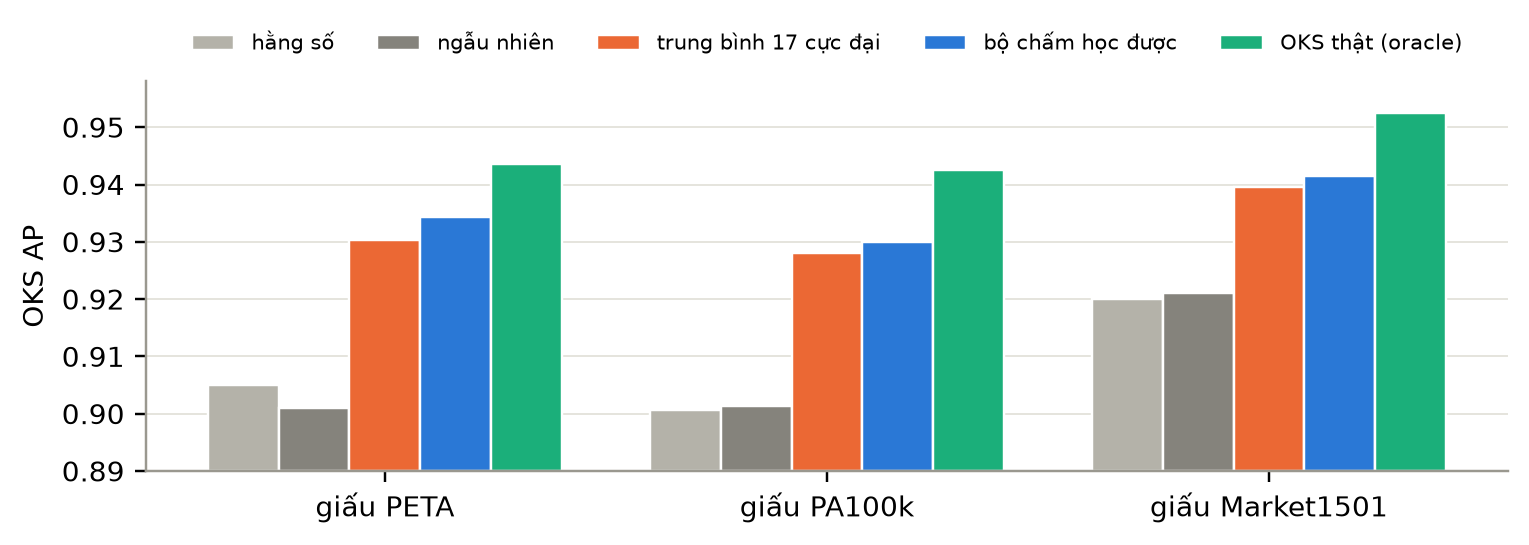
\includegraphics[width=\linewidth]{score_choices.png}
\caption{AP trên ba miền giấu với cùng toạ độ khớp và năm cách gán điểm tin cậy. Điểm mặc định (trung bình 17 cực đại heatmap) cho phần lớn lợi ích so với điểm hằng số. Bộ chấm học được thu hẹp một phần khoảng cách còn lại tới điểm lý tưởng.}
\label{fig:choices}
\end{figure}

\begin{table}[H]
\centering\small
\begin{tabular}{@{}lcccc@{}}
\toprule
Điểm tin cậy & giấu PETA & giấu PA100k & giấu Market1501 & Trung bình \\
\midrule
Hằng số & 0.9050 & 0.9006 & 0.9200 & 0.9086 \\
Ngẫu nhiên & 0.9009 & 0.9013 & 0.9210 & 0.9077 \\
Trung bình 17 cực đại heatmap (mặc định) & 0.9304 & 0.9281 & 0.9396 & 0.9327 \\
Bộ chấm học được (mục~\ref{sec:rescore}) & 0.9344 & 0.9299 & 0.9415 & 0.9352 \\
OKS thật (lý tưởng) & 0.9436 & 0.9426 & 0.9525 & 0.9462 \\
\bottomrule
\end{tabular}
\caption{AP theo cách gán điểm tin cậy, mô hình huge. Điểm mặc định hơn điểm hằng số 0.024. Điểm lý tưởng còn hơn điểm mặc định 0.0132, 0.0145 và 0.0129 trên ba bộ.}
\label{tab:choices}
\end{table}

Hai kết luận rút ra. Thứ nhất, điểm tin cậy đóng góp một phần đáng kể của AP: điểm mặc định hơn điểm hằng số 0.024. Thứ hai, điểm mặc định còn xa điểm lý tưởng. Khoảng cách 0.013 đến 0.015 lớn hơn mức tăng của gộp mô hình ở mục~\ref{sec:lodo}, mà không cần đụng vào toạ độ khớp. Tương quan thứ hạng Spearman giữa điểm mặc định và OKS chỉ ở mức vừa: 0.52 trên PETA, 0.36 trên PA100k và 0.44 trên Market1501.

\subsection{Vì sao điểm mặc định chưa tốt}

Hình~\ref{fig:hist} cho thấy phân bố OKS của từng người trên ba miền giấu lệch mạnh về phía 1. Trung vị OKS là khoảng 0.97, kèm một đuôi các dự đoán sai nặng. Trực giác đầu tiên là điểm tin cậy tốt phải tách đuôi này khỏi phần còn lại. Phép đo ở mục~\ref{sec:rescore} cho thấy trực giác này chỉ đúng một phần nhỏ.

\begin{figure}[H]
\centering
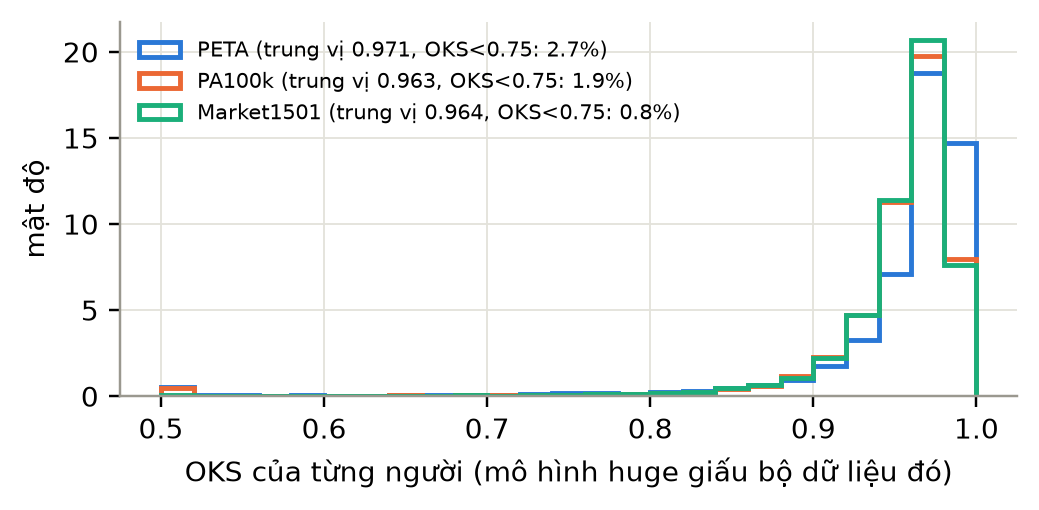
\includegraphics[width=0.66\linewidth]{oks_hist.png}
\caption{Phân bố OKS của từng người với mô hình huge giấu từng bộ dữ liệu. Phần lớn dự đoán gần như đúng, nhưng có một đuôi dài các dự đoán sai nặng mà điểm tin cậy cần xếp xuống cuối.}
\label{fig:hist}
\end{figure}

\begin{figure}[H]
\centering
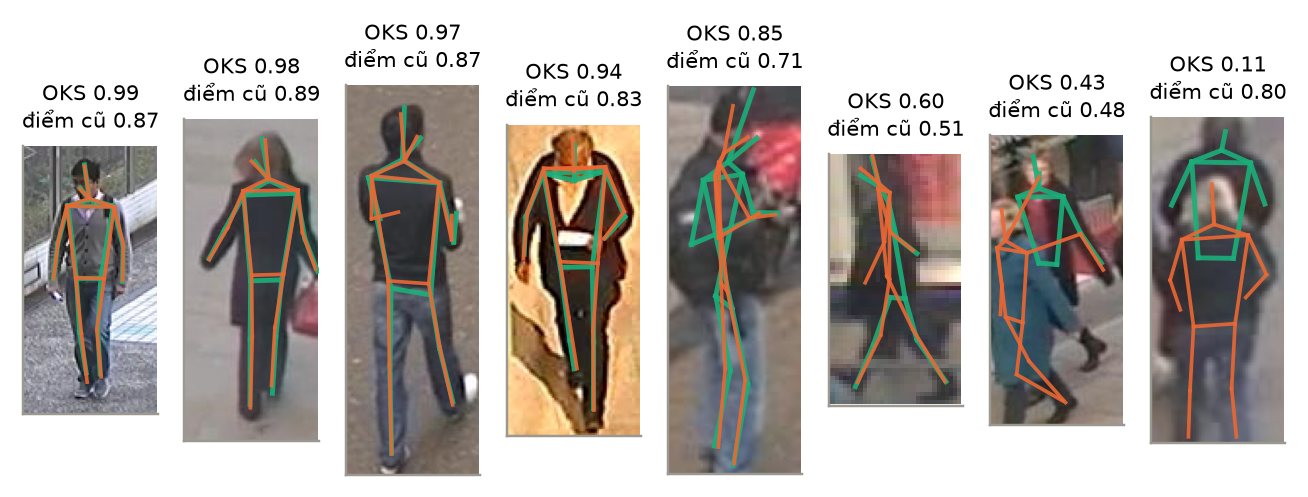
\includegraphics[width=\linewidth]{examples.png}
\caption{Nhãn (xanh lá) và dự đoán của mô hình huge giấu PETA (cam), xếp từ OKS cao tới thấp, cùng điểm tin cậy mặc định. Ảnh cuối là một lỗi điển hình trong ảnh giám sát. Mô hình ước lượng tư thế của người đứng trước thay cho người được gán nhãn phía sau, với OKS 0.11 nhưng điểm tin cậy mặc định 0.80, cao hơn nhiều dự đoán đúng.}
\label{fig:examples}
\end{figure}

Hình~\ref{fig:examples} minh hoạ điểm yếu của điểm mặc định. Trung bình 17 cực đại heatmap đo mức tự tin của mô hình rằng có một khớp ở đâu đó, chứ không đo việc khớp đó có thuộc đúng người được gán nhãn hay không. Ở ảnh cuối, mô hình tìm thấy rất rõ một bộ khung người, chỉ là của người khác. Điểm mặc định cho dự đoán này 0.80, cao hơn nhiều dự đoán có OKS trên 0.9. Tuy vậy, các ca hỏng như thế quá hiếm để chiếm phần lớn giá trị của điểm tin cậy: một oracle chỉ đẩy mọi dự đoán có OKS dưới 0.5 xuống cuối danh sách tăng AP 0.0039, 0.0008 và 0.0005 trên ba bộ, một phần nhỏ của mức tăng mà điểm lý tưởng mang lại. Không bộ nào có quá 1\% số dự đoán dưới OKS 0.5.

%=====================================================================
\section{Học lại điểm tin cậy}
\label{sec:rescore}

\paragraph{Vấn đề.} Điểm tin cậy cần xếp hạng các dự đoán theo OKS thật, nhưng điểm mặc định chỉ dùng một thống kê của heatmap.

\paragraph{Khoảng trống.} Các công thức đơn giản thay thế, đánh giá trên đặc trưng của miền giấu, không tốt hơn trung bình thường: trung bình các cực đại trên 0.2 theo cách của mmpose, trung bình nhân, cực đại nhỏ nhất, trung bình 5 cực đại nhỏ nhất và trung bình có trọng số theo $1/\sigma_k^2$ đều ngang hoặc kém điểm mặc định. Ngoại lệ duy nhất là bỏ hai kênh tai, phân tích ở mục~\ref{sec:ears}. CCNet~\cite{ccnet} học điểm từ đặc trưng bên trong mạng, nhưng cách này cần sửa mô hình và huấn luyện lại một nhánh mới.

\paragraph{Thuộc tính cần có.} Bộ chấm phải học được từ dữ liệu, chỉ dùng thông tin có sẵn ở đầu ra của mô hình đã đóng gói, chạy được với numpy trong môi trường chấm, và được kiểm chứng trên miền không dùng để huấn luyện nó.

\paragraph{Ý tưởng cốt lõi.} Heatmap chứa nhiều thông tin về độ bất định hơn một con số cực đại. Hình dạng của đỉnh, mức độ đồng thuận giữa ảnh gốc và ảnh lật, và mức độ đồng thuận giữa hai mô hình đều là dấu hiệu của dự đoán đáng tin hay không. Một bộ hồi quy học ánh xạ từ các dấu hiệu này sang OKS, huấn luyện trên dự đoán của mô hình ở những bộ dữ liệu mà chính mô hình đó chưa thấy.

\subsection{Đặc trưng}

Với mỗi người, chúng tôi tính 87 đặc trưng từ các heatmap mà chương trình suy luận đã tạo ra.

\begin{itemize}[leftmargin=1.4em]
\item 17 cực đại của heatmap trung bình, đúng giá trị mà điểm mặc định dùng.
\item 17 khoảng cách, tính bằng ô lưới heatmap, giữa toạ độ giải mã từ ảnh gốc và từ ảnh lật, đo sự bất đồng của kiểm tra lật.
\item 17 tỉ số giữa tổng khối của heatmap và cực đại của nó. Tỉ số lớn cho biết heatmap trải rộng hoặc có nhiều đỉnh.
\item 17 độ lệch chuẩn không gian của heatmap quanh trọng tâm của nó.
\item Logarit diện tích khung và tỉ lệ rộng trên cao của khung.
\item Với bản gộp, thêm 17 khoảng cách giữa toạ độ giải mã từ heatmap của large và của huge.
\end{itemize}

Các khoảng cách và độ lệch chuẩn được lấy $\log(1+\cdot)$ để giảm ảnh hưởng của giá trị ngoại lai.

\subsection{Bộ hồi quy và giao thức huấn luyện}

Mục tiêu hồi quy là OKS thật của từng người, tính bằng đúng công thức chấm của cuộc thi. Bộ hồi quy là gradient boosting dựa trên histogram~\cite{friedman,lightgbm} với 150 cây, mỗi cây tối đa 7 lá, learning rate 0.05, tối thiểu 100 mẫu một lá và không dùng dừng sớm. Cấu hình này được chọn sau khi thử một cấu hình lớn hơn (15 lá, 300 cây) trên chính các fold giấu, nên kết quả mang một hiệu ứng chọn nhỏ; hai cấu hình chênh nhau 0.0003 trung bình. Chúng tôi cũng thử hồi quy tuyến tính Ridge và một MLP một tầng ẩn.

Bộ chấm được đánh giá theo cùng giao thức giấu từng bộ dữ liệu. Đặc trưng và OKS của mỗi bộ được tính bằng mô hình tư thế chưa thấy bộ đó. Bộ chấm được huấn luyện trên đặc trưng của hai bộ và chấm AP trên bộ thứ ba. Bộ chấm dùng khi nộp bài được huấn luyện lại trên đặc trưng của cả ba bộ.

\subsection{Xuất sang numpy}

Môi trường chấm không có scikit-learn. Chúng tôi xuất 150 cây thành sáu mảng numpy kích thước 150×13 (chỉ số đặc trưng, ngưỡng, nút con trái, nút con phải, cờ lá, giá trị lá) và một giá trị gốc. Khi suy luận, mọi cây được duyệt đồng thời bằng các phép chỉ số mảng, tối đa bằng độ sâu của cây. Sai khác lớn nhất giữa bản numpy và scikit-learn trên 5000 mẫu là $1.6\cdot10^{-15}$. Tệp bộ chấm nặng 82 KB.

\subsection{Kết quả}

\begin{table}[H]
\centering\small
\begin{tabular}{@{}lcccc@{}}
\toprule
Bộ chấm (mô hình huge) & giấu PETA & giấu PA100k & giấu Market1501 & Trung bình \\
\midrule
Điểm mặc định & 0.9304 & 0.9281 & 0.9396 & 0.9327 \\
MLP một tầng ẩn & 0.9266 & 0.9252 & 0.9368 & 0.9295 \\
Ridge, toàn bộ đặc trưng & 0.9311 & 0.9299 & 0.9413 & 0.9341 \\
Ridge, cực đại và lệch lật & 0.9328 & 0.9297 & 0.9411 & 0.9345 \\
Cây tăng cường, cấu hình lớn (15 lá, 300 cây) & 0.9338 & 0.9293 & 0.9415 & 0.9349 \\
Cây tăng cường, cấu hình nộp bài & 0.9344 & 0.9299 & 0.9415 & 0.9352 \\
\bottomrule
\end{tabular}
\caption{AP trên ba miền giấu với các bộ chấm khác nhau, cùng toạ độ khớp. Cây tăng cường cấu hình nộp bài tăng ở cả ba miền (+0.0040, +0.0018, +0.0019). MLP không được tinh chỉnh siêu tham số, nên chúng tôi không kết luận gì từ nó.}
\label{tab:rescore}
\end{table}

Bảng~\ref{tab:rescore} cho thấy cây tăng cường tăng ở cả ba miền giấu. Lấy mẫu lại người bằng bootstrap với mô hình cố định cho sai số chuẩn 0.0005, 0.0003 và 0.0002 của ba mức tăng, nên chúng vượt xa nhiễu lấy mẫu. So với điểm lý tưởng, bộ chấm lấy lại 30\%, 12\% và 15\% mức tăng có thể. Tương quan thứ hạng với OKS tăng từ 0.52 lên 0.63 trên PETA, từ 0.36 lên 0.43 trên PA100k và từ 0.44 lên 0.48 trên Market1501. Với bản gộp large và huge, bộ chấm 87 đặc trưng tăng AP từ 0.9353 lên 0.9368 (+0.0025, +0.0006, +0.0015 trên ba miền).

\begin{figure}[H]
\centering
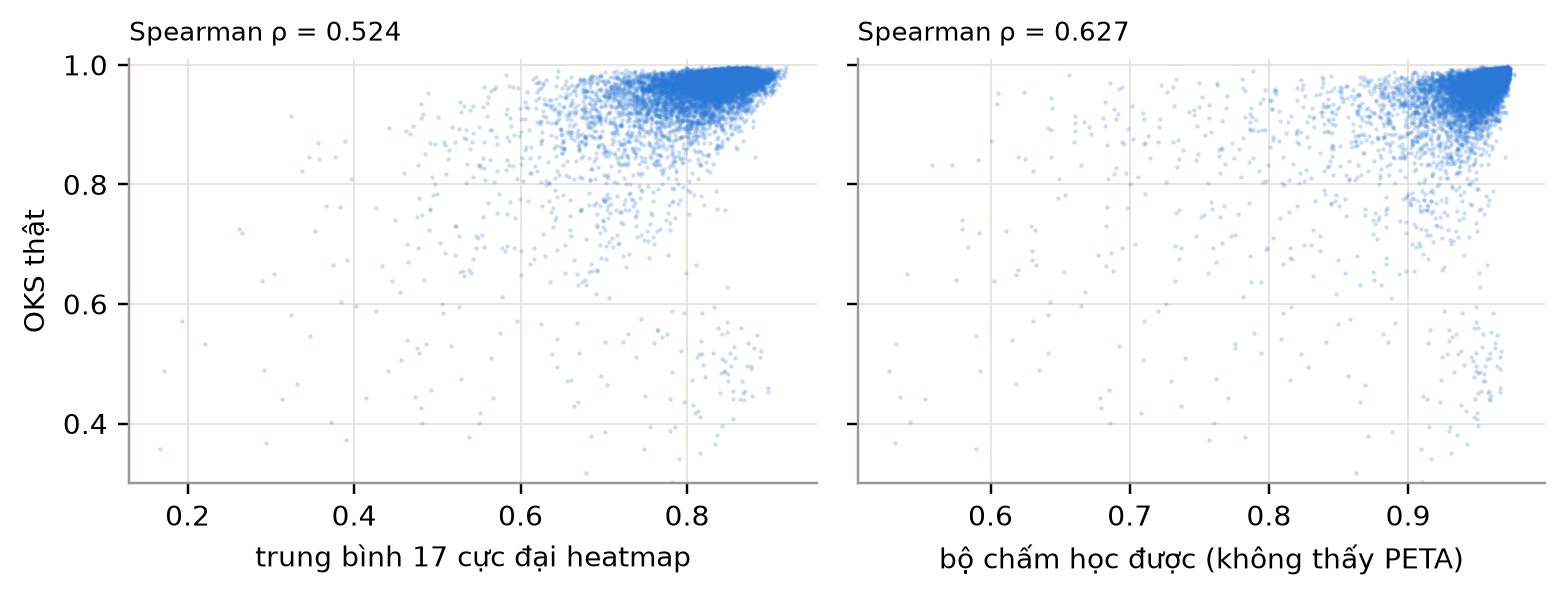
\includegraphics[width=\linewidth]{scatter.png}
\caption{Điểm tin cậy và OKS thật trên PETA giấu. Trái, điểm mặc định. Phải, bộ chấm học được trên PA100k và Market1501. Tương quan thứ hạng tăng từ 0.524 lên 0.627.}
\label{fig:scatter}
\end{figure}

\paragraph{Bộ chấm dựa vào đâu.} Chúng tôi huấn luyện lại bộ chấm, mỗi lần bỏ một nhóm đặc trưng (Bảng~\ref{tab:dropcol}). Bỏ bất kỳ nhóm nào cũng chỉ làm AP trung bình thay đổi tối đa 0.0005, nên các đặc trưng phần lớn trùng thông tin. Đặc biệt, đặc trưng kích thước khung không đóng vai trò nhận diện bộ dữ liệu, một mối lo hợp lý vì mọi khung của Market1501 có cùng kích thước.

\begin{table}[H]
\centering\small
\begin{tabular}{@{}lcccc@{}}
\toprule
Bộ chấm cấu hình nộp bài & giấu PETA & giấu PA100k & giấu Market1501 & Trung bình \\
\midrule
đủ đặc trưng & 0.9344 & 0.9299 & 0.9415 & 0.9353 \\
bỏ 17 cực đại & 0.9339 & 0.9297 & 0.9409 & 0.9348 \\
bỏ độ lệch lật & 0.9343 & 0.9297 & 0.9415 & 0.9352 \\
bỏ tỉ số khối trên đỉnh & 0.9344 & 0.9300 & 0.9415 & 0.9353 \\
bỏ độ lệch chuẩn không gian & 0.9345 & 0.9298 & 0.9415 & 0.9353 \\
bỏ kích thước khung & 0.9343 & 0.9298 & 0.9416 & 0.9352 \\
\bottomrule
\end{tabular}
\caption{Bộ chấm huấn luyện lại khi bỏ từng nhóm đặc trưng (mô hình huge, giấu bộ dữ liệu ở cả hai tầng).}
\label{tab:dropcol}
\end{table}

\subsection{Phần lớn lợi ích là sửa điểm mặc định}
\label{sec:ears}

Điểm mặc định là trung bình cực đại của cả 17 kênh heatmap, gồm hai kênh tai mà PoseTrack không bao giờ gán nhãn (tỉ lệ có nhãn bằng 0 ở cả ba bộ) và chỉ số không bao giờ chấm. Độ tin cậy của hai kênh này không nói gì về các khớp được chấm. Chỉ cần lấy trung bình 15 cực đại còn lại, AP tăng 0.0035, 0.0015 và 0.0018 trên ba bộ, tức phần lớn mức tăng của bộ chấm học được. Bộ chấm học được chỉ còn hơn công thức này 0.0005, 0.0003 và 0.0001, khoảng hai sai số chuẩn trở xuống (mỗi sai số khoảng 0.0002). Hình~\ref{fig:thr} cho thấy hai cách chấm đi cùng nhau ở từng ngưỡng. Lợi thế của bộ chấm học được vì vậy chủ yếu không nằm ở cây, mà ở chỗ cây đã học cách bỏ qua các kênh không được chấm. Phát hiện này cũng giải thích một phần vì sao gộp thêm mô hình làm điểm tốt hơn: trung bình nhiều mô hình làm nhiễu của các kênh tai nhỏ đi.

\subsection{Bộ chấm giúp ở ngưỡng nào}

Hình~\ref{fig:thr} tách mức tăng AP theo 10 ngưỡng OKS cho từng bộ. Trên PA100k và Market1501, 79\% và 78\% mức tăng của điểm lý tưởng nằm ở ngưỡng 0.95, và gần như toàn bộ mức tăng của bộ chấm học được cũng ở đó; trên PA100k, bộ chấm còn hơi âm ở mọi ngưỡng tới 0.85. Trên PETA, mức tăng trải đều hơn: 47\% của điểm lý tưởng và khoảng 40\% của bộ chấm nằm ở 0.95. PETA cũng là bộ có nhiều lỗi nhầm trái phải nhất (mục~\ref{sec:errors}), loại lỗi mà điểm tin cậy có thể đẩy xuống ở mọi ngưỡng, khớp với việc oracle đẩy dự đoán hỏng xuống cuối có ích nhất ở PETA.

\begin{figure}[H]
\centering
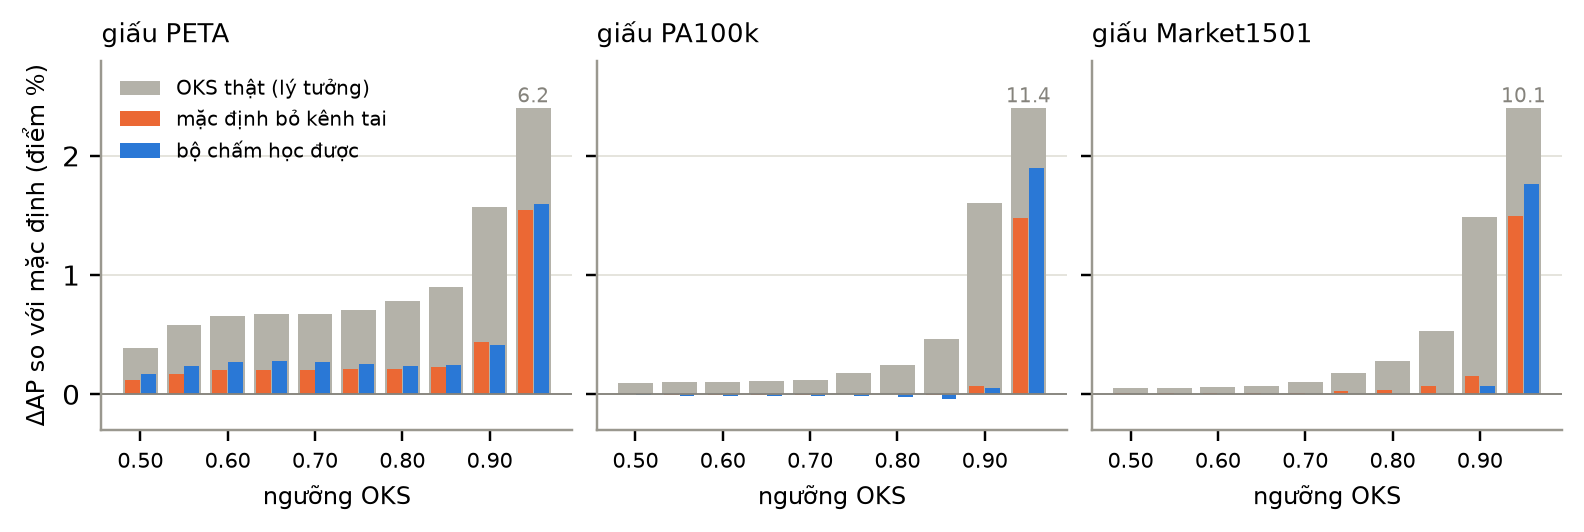
\includegraphics[width=\linewidth]{per_threshold.png}
\caption{Mức tăng AP so với điểm mặc định theo từng ngưỡng OKS, mỗi ô là một miền giấu (mô hình huge, giữ nguyên toạ độ khớp). Xám: OKS thật làm điểm (cắt ở trục, giá trị ghi trên cột). Cam: điểm mặc định bỏ hai kênh tai. Xanh: bộ chấm học được. AP là trung bình 10 ngưỡng, nên tăng 1.6 điểm ở một ngưỡng chỉ thêm 0.16 điểm AP.}
\label{fig:thr}
\end{figure}

Phân tích ở mục~\ref{sec:metric} giải thích hiện tượng này. Ở ngưỡng thấp, hầu hết dự đoán đều đúng ($f_t$ gần 1), nên thứ tự của chúng gần như không quan trọng. Ở ngưỡng 0.90, khoảng 91\% đến 93\% dự đoán được tính là đúng. Ở ngưỡng 0.95, tỉ lệ này giảm còn 69\% đến 76\%. Đây là ngưỡng có tỉ lệ dự đoán sai lớn nhất, nên việc tách dự đoán đúng khỏi dự đoán sai bằng điểm tin cậy có giá trị lớn nhất ở đây. Với người có kích thước trung vị của PETA (khung cao 149 pixel), độ tương đồng 0.95 ở vai cho phép sai khoảng 5 pixel, chưa tới hai ô của heatmap 64×48. Điểm tin cậy vì vậy cần phân biệt các dự đoán rất tốt với các dự đoán chỉ tốt, một nhiệm vụ tinh hơn nhiều so với loại bỏ các dự đoán hỏng.

\subsection{Tương quan thứ hạng không đủ để mô tả chất lượng điểm}

Để đặt các bộ chấm vào bối cảnh, chúng tôi tạo các điểm tin cậy tổng hợp bằng cách cộng nhiễu Gauss với độ lệch chuẩn tăng dần vào OKS thật, rồi đo tương quan Spearman và AP của chúng (Hình~\ref{fig:noise}).

\begin{figure}[H]
\centering
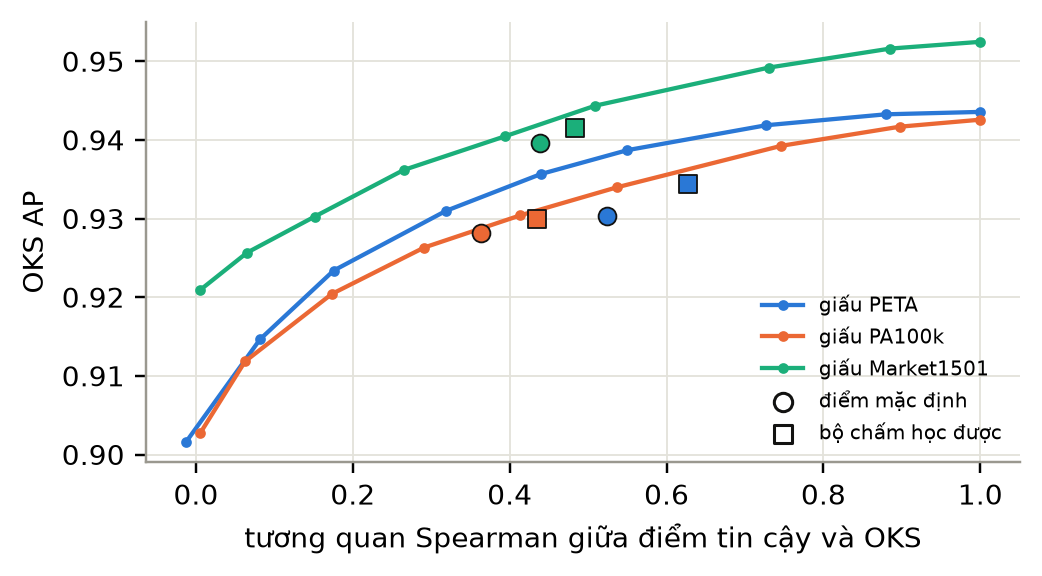
\includegraphics[width=0.68\linewidth]{noise_curve.png}
\caption{AP theo tương quan Spearman của điểm tin cậy tổng hợp (OKS cộng nhiễu Gauss), mỗi đường là một miền giấu. Hình tròn là điểm mặc định, hình vuông là bộ chấm học được. Cả hai nằm dưới đường cong, nên ở cùng mức tương quan, lỗi của chúng gây hại nhiều hơn nhiễu ngẫu nhiên.}
\label{fig:noise}
\end{figure}

AP tăng theo tương quan theo dạng lõm. Lợi ích lớn nhất đến khi tương quan đi từ 0 tới khoảng 0.4. Điểm mặc định và bộ chấm học được đều nằm dưới đường cong của miền tương ứng. Ở cùng một mức tương quan thứ hạng, điểm của chúng cho AP thấp hơn điểm nhiễu ngẫu nhiên. Nhiễu Gauss cộng vào OKS gây lỗi đều trên toàn dải, trong khi lỗi của điểm thật có cấu trúc. Một giả thuyết, chúng tôi chưa đo trực tiếp, là điểm thật thường xếp sai ở vùng OKS cao, đúng vùng mà ngưỡng 0.95 cắt qua. Nếu đúng, cải thiện tương quan tổng thể chưa chắc cải thiện AP tương xứng, và một mục tiêu huấn luyện tập trung vào vùng OKS cao có thể hiệu quả hơn hồi quy bình phương trên toàn dải. Đường nhiễu Gauss chỉ là một mốc tham chiếu, không phải mô hình lỗi đúng của điểm thật.

\begin{ghichu}
Bộ chấm lại điểm tin cậy là một thành phần độc lập với mô hình tư thế. Nó không thay đổi toạ độ khớp nào, nên không thể làm hỏng độ chính xác định vị, và nó chỉ được huấn luyện và kiểm chứng trên dự đoán của mô hình ở các miền mà mô hình chưa thấy.
\end{ghichu}

%=====================================================================
\section{Phân tích lỗi}
\label{sec:errors}

\subsection{Khớp nào khó nhất}

Hình~\ref{fig:joints} đo độ tương đồng của từng khớp, là thành phần $\exp(-d^2/2s^2\kappa^2)$ của OKS, trung bình trên các khớp có nhãn của mô hình huge giấu từng bộ dữ liệu.

\begin{figure}[H]
\centering
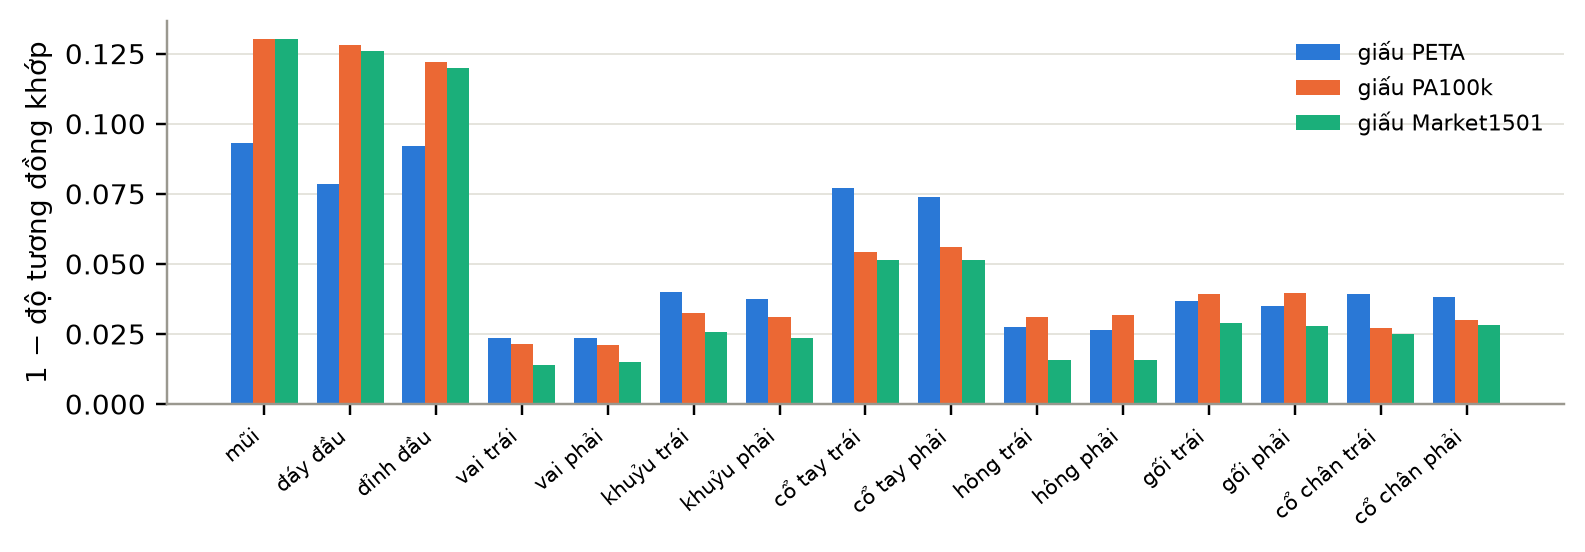
\includegraphics[width=\linewidth]{joints.png}
\caption{Phần mất độ tương đồng của từng khớp trên ba miền giấu. Ba điểm vùng đầu mất nhiều nhất, tiếp theo là cổ tay. Vai và hông là các khớp dễ nhất.}
\label{fig:joints}
\end{figure}

Ba điểm vùng đầu (mũi, đáy đầu, đỉnh đầu) mất 0.08 đến 0.13, gấp ba đến năm lần vai và hông (0.014 đến 0.032). Có hai lý do. Hằng số $\sigma$ của ba điểm này nhỏ nhất (0.025 và 0.026), nên cùng một sai số pixel bị phạt nặng hơn nhiều so với hông ($\sigma=0.107$). Ngoài ra đáy đầu và đỉnh đầu không có trong COCO, nên mô hình phải học chúng chỉ từ dữ liệu UPAR, và vị trí của chúng phụ thuộc vào quy ước gán nhãn hơn là vào một mốc giải phẫu rõ ràng. PETA là ngoại lệ, với điểm vùng đầu tốt hơn hai miền còn lại, nhưng cổ tay kém hơn (0.074 đến 0.077). Cổ tay là khớp nhỏ và di chuyển nhiều.

\subsection{Kích thước người}

\begin{figure}[H]
\centering
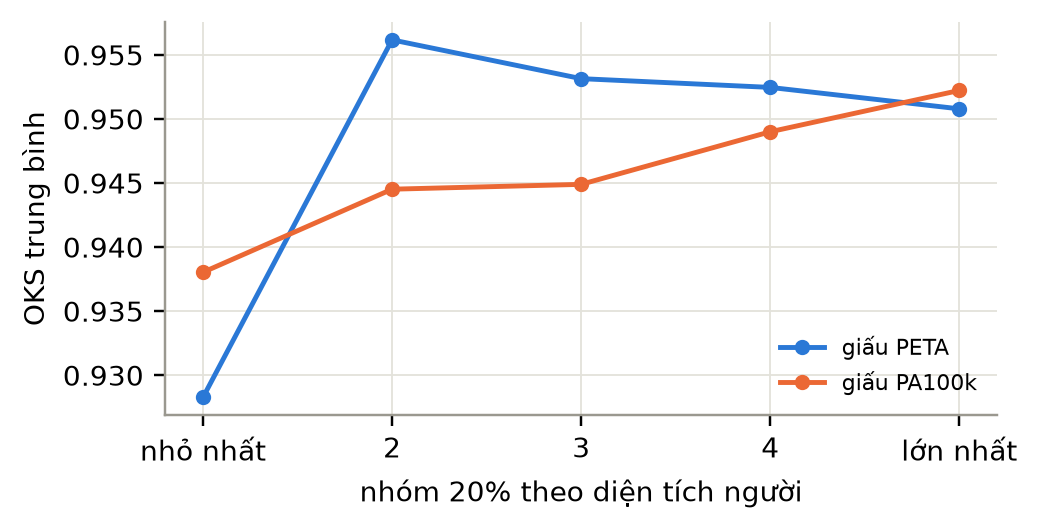
\includegraphics[width=0.62\linewidth]{size.png}
\caption{OKS trung bình theo năm nhóm diện tích người bằng nhau về số lượng, trên PETA và PA100k giấu. Nhóm nhỏ nhất kém rõ rệt. Market1501 không được vẽ vì gần như mọi khung là toàn bộ ảnh 128×64.}
\label{fig:size}
\end{figure}

Hình~\ref{fig:size} cho thấy nhóm 20\% người nhỏ nhất theo diện tích khung có OKS thấp hơn (0.937 so với 0.953 của phần còn lại ở PETA, 0.938 so với 0.948 ở PA100k). Ở PETA, nhóm nhỏ nhất có diện tích khung dưới 6144 pixel vuông, cỡ một khung 48×128. Sau khi phóng lên 256×192, các ảnh này mờ và thiếu chi tiết để phân biệt khớp. Đây cũng là lý do log diện tích khung được đưa vào bộ chấm.

\subsection{Nhầm trái và phải}

Hình~\ref{fig:resid} cho thấy các người có OKS dưới 0.5 nhưng vẫn được bộ chấm xếp vào nửa trên. Trên hình, khung xương dự đoán và khung xương nhãn gần như trùng nhau. Chúng tôi kiểm tra giả thuyết rằng mô hình nhầm người quay mặt với người quay lưng. Khi đó mọi khớp bên trái được gán sang bên phải và ngược lại, nên khung xương vẽ ra trông giống nhau nhưng từng khớp đều sai. Ronchi và Perona~\cite{ronchi} gọi loại lỗi này là \textbf{inversion} (tạm dịch: nhầm trái phải trong cùng một người), phân biệt với \textbf{swap} (lấy khớp của người khác).

\begin{figure}[H]
\centering
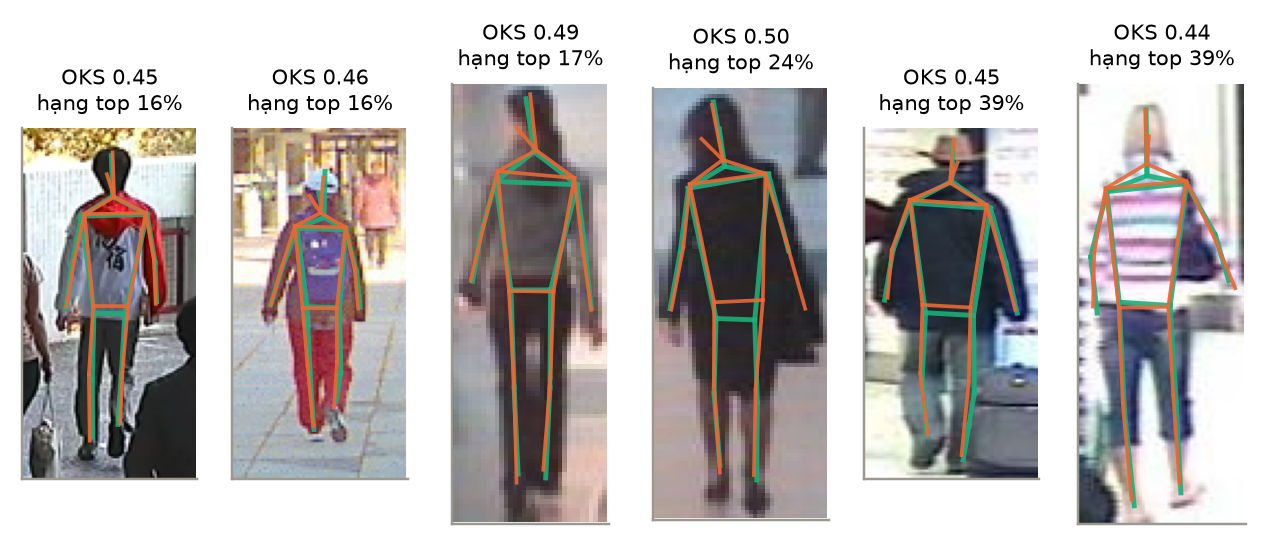
\includegraphics[width=\linewidth]{residuals.png}
\caption{Các người trên PETA giấu có OKS dưới 0.5 nhưng được bộ chấm học được xếp hạng cao. Khung xương dự đoán (cam) và nhãn (xanh lá) trông trùng nhau vì hình vẽ không phân biệt trái và phải. Phần lớn các ca này là nhầm hướng người, có OKS trên 0.8 sau khi hoán đổi trái phải.}
\label{fig:resid}
\end{figure}

\begin{table}[H]
\centering\small
\begin{tabular}{@{}lccc@{}}
\toprule
& giấu PETA & giấu PA100k & giấu Market1501 \\
\midrule
Số người có OKS dưới 0.5 & 97 & 187 & 21 \\
Trong đó, OKS trên 0.8 sau khi hoán đổi trái phải & 51 (53\%) & 55 (29\%) & 12 (57\%) \\
Tỉ lệ mọi người mà hoán đổi tăng OKS hơn 0.2 & 1.3\% & 0.6\% & 0.2\% \\
AP, điểm mặc định & 0.9304 & 0.9281 & 0.9396 \\
AP khi sửa các ca nhầm, điểm mặc định & 0.9469 & 0.9323 & 0.9400 \\
AP khi sửa các ca nhầm, OKS thật làm điểm & 0.9545 & 0.9465 & 0.9525 \\
\bottomrule
\end{tabular}
\caption{Nhầm trái và phải trên ba miền giấu và số AP mà chúng làm mất. Gộp ba bộ, 39\% số dự đoán dưới OKS 0.5 là nhầm trái phải.}
\label{tab:swap}
\end{table}

Bảng~\ref{tab:swap} xác nhận giả thuyết. Ở PETA và Market1501, hơn một nửa số dự đoán có OKS dưới 0.5 trở thành dự đoán tốt (OKS trên 0.8) chỉ bằng cách hoán đổi trái phải; ở PA100k là 29\%. Tính trên mọi người, nhầm trái phải chỉ chiếm 0.2\% đến 1.3\%. Nhưng thay các dự đoán đó bằng bản đã hoán đổi, giữ nguyên điểm mặc định, sẽ tăng AP 0.0165 trên PETA, nhiều hơn toàn bộ khoảng cách tới điểm tin cậy lý tưởng ở đó, và 0.0042 và 0.0004 trên hai bộ còn lại.

Lỗi này khó phát hiện từ đầu ra. Mô hình rất chắc chắn về vị trí các khớp, chỉ sai về nhãn trái phải. Kiểm tra lật cũng không lộ ra nó: lật ảnh không đổi việc người đó quay mặt hay quay lưng, nên mô hình mắc cùng một lỗi ở cả hai lần chạy và đặc trưng độ lệch lật vẫn thấp. Sau khi nộp bài, chúng tôi thử hai cách phát hiện trên dự đoán giấu bộ dữ liệu, và cả hai đều thất bại. Quy tắc ``mũi được nhìn rõ nhưng vai và hông xếp theo thứ tự nhìn từ sau lưng'' gắn cờ khoảng 45\% số người nhưng chỉ khoảng 2\% trong số đó là nhầm thật, vì heatmap mũi vẫn tự tin cả khi người quay lưng. Một bộ phân loại cây tăng cường trên đặc trưng heatmap cộng hình học tư thế, huấn luyện giấu bộ dữ liệu, chỉ đạt độ chính xác tối đa 10\% ở các ứng viên đứng đầu, và hoán đổi các ứng viên đó làm AP giảm. Sửa lỗi này vì vậy cần tín hiệu về hướng người lấy từ chính ảnh, tức là phải huấn luyện thêm. Chúng tôi cũng chưa kiểm tra bao nhiêu ca là nhãn bị gán ngược, điều có thể xảy ra ở ảnh độ phân giải thấp.

%=====================================================================
\section{Kết quả trên tập chấm ẩn}
\label{sec:test}

\begin{figure}[H]
\centering
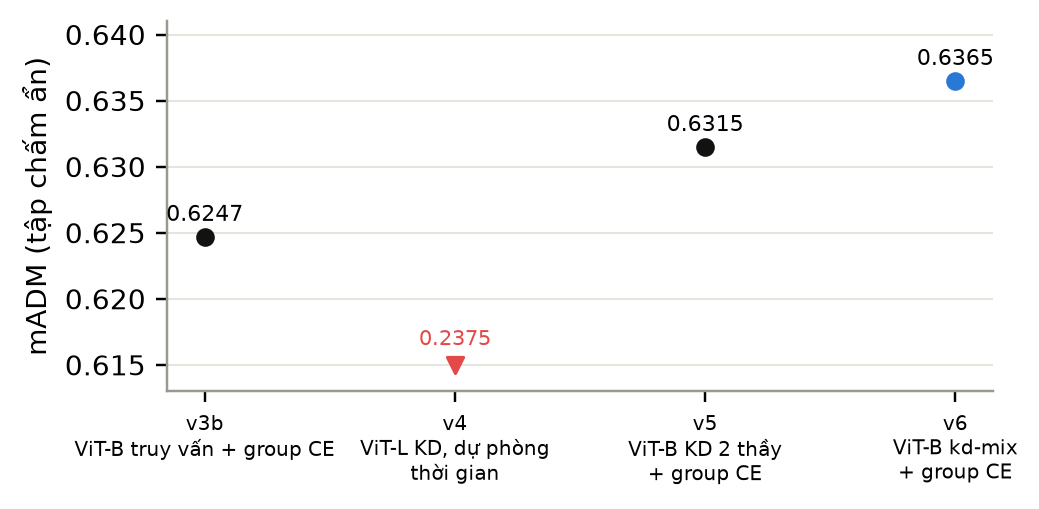
\includegraphics[width=\linewidth]{leaderboard.png}
\caption{OKS AP trên tập chấm ẩn. Trái, bài mẫu không tinh chỉnh so với bài tinh chỉnh đầu tiên. Phải, các bước sau tinh chỉnh.}
\label{fig:lb}
\end{figure}

\begin{table}[H]
\centering\small
\begin{tabularx}{\linewidth}{@{}llXcc@{}}
\toprule
Bài & Mô hình & Thay đổi & Tập chấm & Dự báo từ miền giấu \\
\midrule
mẫu & ViTPose+ S & không tinh chỉnh (bài của ban tổ chức) & 0.6238 & \\
v1 & ViTPose+ B & tinh chỉnh trên hai bộ dữ liệu & 0.8813 & \\
v2 & ViTPose+ L & đổi cỡ, ba bộ dữ liệu, 5 epoch (ba yếu tố) & 0.8939 & \\
v4 & ViTPose+ H & huge thay large & 0.8958 & +0.0010 \\
v3 & L + H & gộp heatmap & 0.8977 & +0.0026 \\
v6 & L + H & + bộ chấm điểm & 0.8992 & +0.0015 (0.0006 đến 0.0025) \\
\bottomrule
\end{tabularx}
\caption{Các bài nộp Track 3. Cột cuối là mức tăng trung bình trên ba miền giấu của cùng thay đổi. Ba bước cuối mỗi bước đổi một yếu tố và đều cùng chiều với giao thức.}
\label{tab:lb}
\end{table}

Bảng~\ref{tab:lb} tóm tắt các bài nộp. Mốc so sánh có ý nghĩa là mô hình base tinh chỉnh (v1); bài mẫu của ban tổ chức chịu độ lệch định nghĩa điểm vùng đầu ở mục~\ref{sec:lodo}. Ba bước cuối mỗi bước đổi một yếu tố, và cả ba cùng chiều với giao thức. Bộ chấm điểm thêm 0.0015, nằm trong khoảng 0.0006 đến 0.0025 của nó trên ba miền giấu. Điều này nhất quán với việc giao thức đại diện được cho tập chấm ở loại thay đổi này, nhưng chỉ là một quan sát.

\paragraph{Bộ chấm gặp đặc trưng chưa được kiểm chứng.} Bộ chấm nộp bài được huấn luyện trên heatmap của các mô hình giấu bộ dữ liệu học 2 epoch, nhưng được áp lên mô hình học 5 epoch trên toàn bộ dữ liệu, mà heatmap có thể sắc hơn. Chúng tôi đã kiểm tra đường chạy của mã, nhưng chưa kiểm tra dịch chuyển phân bố này.

\paragraph{Kiểm tra gói nộp.} Trước khi nộp v6, chúng tôi chạy \texttt{run.py} thật với mô hình large và huge giấu PETA, xuất sang TorchScript, và bộ chấm huấn luyện không có PETA, trên toàn bộ 10.314 người của PETA. AP từ \texttt{run.py} tăng từ 0.9351 lên 0.9377, khớp với giao thức thẩm định. Đặc trưng do \texttt{run.py} tính có tương quan 0.98 đến 1.00 với đặc trưng lúc huấn luyện, với sai khác nhỏ do chạy fp16 thay cho bf16. Gói nộp thật được chạy thêm trong môi trường PyTorch 2.4.1 giống máy chấm. Toạ độ khớp trùng với bài v3 trên 300 ảnh, sai khác 0 pixel, lời gọi với nhiều khung trong một ảnh chạy đúng, và thời gian khoảng 45 ms một ảnh trên A100. Với 30.245 khung, thời gian ước lượng khoảng 23 phút, trong giới hạn 2 giờ.

\paragraph{Khoảng cách giữa miền giấu và tập chấm.} AP trên tập chấm (khoảng 0.90) thấp hơn AP trên các miền giấu (khoảng 0.93). Tập chấm là một miền khác cả ba bộ dữ liệu huấn luyện, và có thể khó hơn về độ phân giải hoặc mức che khuất. Thứ tự giữa các phương án vẫn được giữ, nên giao thức giấu từng bộ dữ liệu vẫn có ích cho việc chọn phương án dù không dự báo được mức điểm tuyệt đối.

%=====================================================================
\section{Chi phí tính toán và triển khai}
\label{sec:deploy}

\paragraph{Ngân sách.} Giới hạn 7200 giây cho 30.245 khung cho ngân sách trung bình 238 ms một khung, bao gồm đọc ảnh, cắt, chạy mô hình và giải mã. Máy chấm có GPU, nên khác với Track 1 và Track 2, ràng buộc thời gian ở Track 3 cho phép dùng cả hai mô hình lớn nhất cùng lúc. Bảng~\ref{tab:cost} tóm tắt các con số đo được.

\begin{table}[H]
\centering\small
\begin{tabularx}{\linewidth}{@{}Xcc@{}}
\toprule
Cấu hình & Thời gian & Kích thước trọng số \\
\midrule
ViTPose+ L (v2), máy chấm & khoảng 1160 giây cho toàn tập (38 ms một khung) & 0,87 GB \\
ViTPose+ H (v4) & không ghi nhận & 1,80 GB \\
L + H (v3), GPU laptop & khoảng 90 ms một khung & 2,67 GB \\
L + H + bộ chấm (v6), A100, gọi từng ảnh & khoảng 45 ms một khung (ước lượng 23 phút) & 2,67 GB + 82 KB \\
\bottomrule
\end{tabularx}
\caption{Thời gian và kích thước của các cấu hình Track 3. Mọi cấu hình đều nằm trong ngân sách 238 ms một khung. Bộ chấm điểm thêm bốn lần giải mã DARK trên GPU và một lần duyệt cây trên CPU, không đáng kể so với hai mô hình.}
\label{tab:cost}
\end{table}

\paragraph{Ràng buộc của môi trường chấm.} Môi trường chấm chỉ có PyTorch, numpy và Pillow. Ba thành phần của quy trình huấn luyện vì vậy phải viết lại cho bài nộp. Phép affine dùng OpenCV khi huấn luyện được thay bằng nội suy song tuyến tính viết bằng numpy, giữ đúng quy ước pixel của OpenCV. Bộ lọc Gauss và giải mã DARK được viết bằng các phép tích chập và chỉ số của PyTorch. Bộ hồi quy cây được xuất sang numpy như mô tả ở mục~\ref{sec:rescore}. Mỗi gói nộp được kiểm tra bằng cách chạy chính \texttt{run.py} trên ảnh có nhãn, chấm OKS AP của đầu ra và so với kết quả của mã huấn luyện trên cùng ảnh.

\paragraph{Giao diện gọi từng ảnh.} Chương trình chấm gọi hàm dự đoán một lần cho mỗi ảnh, với danh sách các khung của ảnh đó. Mọi khung của một ảnh được xử lý thành một batch. Vì phần lớn ảnh chỉ có một khung, GPU thường chạy với batch 1 hoặc 2, nên thời gian chủ yếu bị chi phối bởi độ trễ của từng lần gọi mô hình chứ không phải thông lượng. Đây là lý do thời gian một khung trên A100 (45 ms) chỉ nhanh hơn GPU laptop khoảng hai lần.

\paragraph{Không có cơ chế dự phòng.} Các gói nộp Track 3 chỉ chạy trên GPU và không có cơ chế dự phòng thời gian. Bài học từ Track 1 và Track 2 là một bài nộp quá giờ thì thất bại và giữ nguyên điểm cũ, còn một bài nộp dự phòng trả về kết quả kém thì thay điểm tốt bằng điểm xấu trên bảng xếp hạng. Hai bài nộp đầu (v1, v2) có kèm một mô hình small chạy trên CPU phòng khi máy chấm không có GPU. Khi đã biết máy chấm có GPU, các bài sau bỏ mô hình này.

%=====================================================================
\section{Thảo luận}

\paragraph{Các hướng đã cân nhắc và bị loại.} Gán nhãn giả trên ảnh chấm là hướng phổ biến nhất trong thích nghi miền cho tư thế~\cite{regda,kim2022}, nhưng bị luật thi cấm rõ ràng. Gán nhãn giả trên ảnh không nhãn của chính ba bộ dữ liệu huấn luyện là hợp lệ, nhưng chỉ thêm dữ liệu từ các miền đã có. Backbone DINOv3 và chưng cất từ mô hình nền tảng bị luật cấm.

\subsection{Thử nghiệm bổ sung sau khi nộp}
\label{sec:extra}

Sau v6, chúng tôi thuê thêm 4 GPU để thử ba hướng còn lại trên fold giấu PETA, mỗi lần chạy 1 đến 2 epoch. Không hướng nào đáng đóng gói.

\paragraph{Ảnh vào 384×288.} Chúng tôi nội suy lưới mã hoá vị trí từ 16×12 lên 24×18, dùng heatmap 96×72 với $\sigma=3$. Large ở 384×288 đạt 0.9330 sau 1 epoch, so với 0.9337 của large ở 256×192; trên fold PA100k là 0.9065 so với 0.9048. Gộp heatmap của large 256 và large 384 (phóng heatmap 64×48 lên 96×72) đạt 0.9366 trên PETA, cao hơn từng mô hình khoảng 0.004. Nhưng khi giữ nguyên điểm tin cậy lấy từ large 256 và huge 256, thêm large 384 vào bản gộp chỉ đổi AP từ 0.9365 sang 0.9366. Toạ độ khớp vì vậy không tốt hơn; phần tăng khi gộp đến từ điểm tin cậy, thứ mà bộ chấm của v6 đã cải thiện.

\paragraph{Thay head.} Giữ backbone large 256×192 và 1 epoch, chúng tôi so head heatmap gốc (0.9324) với ba head khác. Head siêu phân giải, thêm một tầng giải chập để ra heatmap 128×96, đạt 0.9312 với điểm mặc định và 0.9343 khi bỏ kênh tai, đều trong nhiễu. Head SimCC~\cite{simcc}, phân loại toạ độ $x$ và $y$ với hai ô mỗi pixel, đạt 0.9253. Head kết hợp heatmap và SimCC cho 0.9129 khi lấy toạ độ từ SimCC và 0.9324 khi lấy từ heatmap. Lợi thế của SimCC mà tài liệu báo cáo xuất hiện chủ yếu ở ảnh vào rất nhỏ; ở đây khung đã được phóng lên 256×192, và heatmap kết hợp DARK đã đủ chính xác.

\paragraph{Kết luận của các thử nghiệm.} Với các mô hình được luật cho phép, độ chính xác toạ độ khớp đã bão hoà ở ViTPose++ large và huge. Phần còn lại nằm ở điểm tin cậy và ở lỗi nhầm trái phải.

\paragraph{Khoảng cách tới điểm tin cậy lý tưởng.} Bộ chấm học được mới lấy lại 12 đến 30\% khoảng cách giữa điểm mặc định và điểm lý tưởng, và phần lớn phần đó là việc bỏ qua kênh tai. Phần còn lại có thể đến từ thông tin mà heatmap đầu ra không chứa, như việc khung cắt có hai người hay không. Một hướng tiếp theo là dùng đặc trưng bên trong backbone như CCNet, với cái giá là phải huấn luyện thêm một nhánh và đóng gói lại mô hình.

\paragraph{Giới hạn.} Mỗi cấu hình thẩm định chỉ được huấn luyện một lần, và dao động giữa các epoch chỉ là cận dưới của nhiễu huấn luyện. Các mô hình thẩm định học 2 epoch, trong khi mô hình nộp bài học 5 epoch. Phép so trên khớp chung chỉ chạy trên PETA. Dữ liệu giấu bộ dữ liệu có một khung mỗi ảnh, khác một phần tập chấm. Việc dùng ViTPose++ dựa trên cách hiểu luật đã nêu ở mục~\ref{sec:task}.

\paragraph{Tác động xã hội.} Ước lượng tư thế trên video giám sát có thể hỗ trợ việc theo dõi cá nhân. Báo cáo chỉ trình bày kết quả kỹ thuật và không công bố mô hình đã huấn luyện.

%=====================================================================
\section{Kết luận}

Khi khung người được cho sẵn, OKS AP bị chặn giữa tỉ lệ dự đoán đúng và bình phương của nó, và điểm tin cậy quyết định hệ thống nằm ở đâu giữa hai cận. Trên camera giám sát chưa thấy, phần này đáng giá hơn một mô hình thứ hai, và trên hai trong ba bộ dữ liệu gần như toàn bộ nằm ở ngưỡng OKS 0.95. Một bộ chấm học được lấy lại một phần, chủ yếu nhờ bỏ qua các kênh không được chấm. Phần lớn mức tăng ``0.23'' của tinh chỉnh là học định nghĩa điểm khớp vùng đầu, còn nguồn lỗi lớn nhất trên PETA là nhầm trái phải, thứ mà cả điểm tin cậy lẫn kiểm tra lật đều không nhìn thấy. Hệ thống đạt 0.8992 OKS AP trên tập chấm ẩn của UPAR Challenge 2027 Track 3.

%=====================================================================
\begin{thebibliography}{99}\small
\bibitem{coco} T.-Y.~Lin, M.~Maire, S.~Belongie và cộng sự. Microsoft COCO: Common objects in context. \textit{ECCV}, 2014.
\bibitem{posetrack} M.~Andriluka, U.~Iqbal, E.~Insafutdinov và cộng sự. PoseTrack: A benchmark for human pose estimation and tracking. \textit{CVPR}, 2018.
\bibitem{simplebaseline} B.~Xiao, H.~Wu, Y.~Wei. Simple baselines for human pose estimation and tracking. \textit{ECCV}, 2018.
\bibitem{hrnet} K.~Sun, B.~Xiao, D.~Liu, J.~Wang. Deep high-resolution representation learning for human pose estimation. \textit{CVPR}, 2019.
\bibitem{vitpose} Y.~Xu, J.~Zhang, Q.~Zhang, D.~Tao. ViTPose: Simple vision transformer baselines for human pose estimation. \textit{NeurIPS}, 2022.
\bibitem{vitposepp} Y.~Xu, J.~Zhang, Q.~Zhang, D.~Tao. ViTPose++: Vision transformer for generic body pose estimation. \textit{IEEE TPAMI}, 2023.
\bibitem{mae} K.~He, X.~Chen, S.~Xie và cộng sự. Masked autoencoders are scalable vision learners. \textit{CVPR}, 2022.
\bibitem{udp} J.~Huang, Z.~Zhu, F.~Guo, G.~Huang. The devil is in the details: Delving into unbiased data processing for human pose estimation. \textit{CVPR}, 2020.
\bibitem{dark} F.~Zhang, X.~Zhu, H.~Dai, M.~Ye, C.~Zhu. Distribution-aware coordinate representation for human pose estimation. \textit{CVPR}, 2020.
\bibitem{gpose} G.~Papandreou, T.~Zhu, N.~Kanazawa và cộng sự. Towards accurate multi-person pose estimation in the wild. \textit{CVPR}, 2017.
\bibitem{ronchi} M.~R.~Ronchi, P.~Perona. Benchmarking and error diagnosis in multi-instance pose estimation. \textit{ICCV}, 2017.
\bibitem{ccnet} K.~Gu, R.~Chen, X.~Yu, A.~Yao. On the calibration of human pose estimation. \textit{ICML}, 2024.
\bibitem{dekr} Z.~Geng, K.~Sun, B.~Xiao, Z.~Zhang, J.~Wang. Bottom-up human pose estimation via disentangled keypoint regression. \textit{CVPR}, 2021.
\bibitem{regda} J.~Jiang, Y.~Ji, X.~Wang, Y.~Liu, J.~Wang, M.~Long. Regressive domain adaptation for unsupervised keypoint detection. \textit{CVPR}, 2021.
\bibitem{kim2022} D.~Kim, K.~Wang, K.~Saenko, M.~Betke, S.~Sclaroff. A unified framework for domain adaptive pose estimation. \textit{ECCV}, 2022.
\bibitem{simcc} Y.~Li, S.~Yang, P.~Liu và cộng sự. SimCC: A simple coordinate classification perspective for human pose estimation. \textit{ECCV}, 2022.
\bibitem{lightgbm} G.~Ke và cộng sự. LightGBM: A highly efficient gradient boosting decision tree. \textit{NeurIPS}, 2017.
\bibitem{friedman} J.~H.~Friedman. Greedy function approximation: A gradient boosting machine. \textit{Annals of Statistics}, 2001.
\end{thebibliography}

\appendix
\section{Cấu hình chi tiết}

\begin{table}[H]
\centering\small
\begin{tabularx}{\linewidth}{@{}lX@{}}
\toprule
Thành phần & Giá trị (bài nộp v6) \\
\midrule
Mô hình & \texttt{usyd-community/vitpose-plus-large} và \texttt{-huge}, head COCO, TorchScript fp16 \\
Ảnh vào, heatmap & 256×192, 64×48, đệm khung 1.25, tỉ lệ 3:4, affine theo quy ước UDP \\
Huấn luyện & AdamW, lr $5\cdot10^{-5}$, layer decay 0.75, weight decay 0.1, warmup 300 bước, cosine, batch 64, bf16, 5 epoch, cả ba bộ dữ liệu \\
Mục tiêu & Gauss $\sigma=2$ ô lưới, MSE có trọng số khả kiến, nhân 1000 \\
Tăng cường & tỉ lệ $[0.75,1.25]$, dời tâm 8\%, xoay $\pm40°$ (xác suất 0.4), lật 0.5, sáng và tương phản (xác suất 0.8) \\
Suy luận & kiểm tra lật, trung bình heatmap của hai mô hình, DARK với lọc Gauss kích thước 11 \\
Bộ chấm điểm & 87 đặc trưng, gradient boosting 150 cây, 7 lá, lr 0.05, tối thiểu 100 mẫu một lá, xuất numpy \\
\bottomrule
\end{tabularx}
\caption{Cấu hình của bài nộp Track 3 tốt nhất.}
\end{table}

\section{Duyệt cây bằng numpy}

Gọi $T=150$ là số cây, $N$ là số người trong một lời gọi, và \texttt{node} là ma trận $N\times T$ khởi tạo bằng 0 (nút gốc). Ở mỗi vòng lặp, với mọi cặp người và cây chưa tới lá, so đặc trưng \texttt{f[n, feat[t, node]]} với ngưỡng \texttt{thr[t, node]} và chuyển sang nút con trái hoặc phải. Vòng lặp dừng khi mọi phần tử của \texttt{node} là lá, sau tối đa bằng độ sâu lớn nhất của cây. Điểm của người $n$ là giá trị gốc cộng tổng giá trị lá trên 150 cây. Toàn bộ thuật toán gồm các phép chỉ số mảng của numpy, không có vòng lặp theo người hay theo cây.


\section{Tái lập kết quả}

Mã nguồn nằm trong thư mục \texttt{t3/} của kho Track 3. Các bước dưới đây tái lập bộ chấm điểm và gói nộp v6 từ đầu.

\begin{enumerate}[leftmargin=1.6em]
\item Chuẩn bị dữ liệu bằng script của ban tổ chức. Ảnh được đặt dưới thư mục \texttt{data/} theo tên từng bộ dữ liệu.
\begingroup\footnotesize
\begin{verbatim}
python starter/download_datasets.py --data-dir data
\end{verbatim}
\endgroup
\item Huấn luyện sáu mô hình giấu từng bộ dữ liệu (large và huge, ba giá trị của \texttt{--holdout}). Trên một A100, mỗi mô hình huge mất khoảng 15 đến 25 phút.
\begingroup\footnotesize
\begin{verbatim}
python pose.py --model usyd-community/vitpose-plus-huge \
    --holdout peta --epochs 2 --out ../runs/h_lodo_peta
\end{verbatim}
\endgroup
\item Trích đặc trưng trên bộ dữ liệu giấu. Với hai mô hình, lệnh ghi tệp \texttt{feats\_peta\_ens.npz}.
\begingroup\footnotesize
\begin{verbatim}
python rescore_feats.py ../runs/l_lodo_peta,../runs/h_lodo_peta peta
\end{verbatim}
\endgroup
\item Đánh giá bộ chấm theo giao thức giấu từng bộ bằng \texttt{rescore\_eval.py} và \texttt{rescore\_ens\_eval.py}.
\item Huấn luyện bộ chấm cuối trên cả ba bộ và xuất sang numpy. Tệp kết quả được chép vào gói nộp với tên \texttt{assets/rescorer.npz}, và khoá \texttt{"rescorer"} được thêm vào \texttt{config.json}.
\begingroup\footnotesize
\begin{verbatim}
python rescore_export.py ../runs/lodo/feats_{peta,pa100k,market}_ens.npz \
    --out ../runs/lodo/rescorer_ens.npz
\end{verbatim}
\endgroup
\item Mô hình nộp bài được huấn luyện với \texttt{--holdout none --epochs 5} và xuất sang TorchScript fp16 bằng \texttt{export.py} với cờ \texttt{--half}.
\end{enumerate}

\end{document}
